\documentclass[11pt]{article}

\usepackage[margin=2.5cm]{geometry}
\usepackage{graphicx}
\usepackage{amsmath}
\usepackage{amssymb}
\usepackage{booktabs}
\usepackage{hyperref}
\usepackage{caption}
\usepackage{xcolor}
\usepackage{natbib}
\usepackage{float}

\title{Quadratic Maximum Likelihood power-spectrum recovery\\
on GLASS mock weak-lensing catalogues:\\
sky-coverage and depth requirements, and implications for TR1}
\author{Weak Lensing QML pipeline}
\date{\today}

\begin{document}
\maketitle

\begin{abstract}
We test a C++ implementation of the Quadratic Maximum Likelihood (QML) power-spectrum
estimator against the pseudo-$C_\ell$ (PCl, via \texttt{NaMaster}) and an independent
catalogue-based (\texttt{heracles}) estimator, using full-sky log-normal weak-lensing
mock catalogues generated with \texttt{GLASS}. We scan a $3\times3$ grid of galaxy number
density ($n=1,10,20\ \mathrm{arcmin}^{-2}$) and survey footprint (three Galactic+ecliptic
cuts giving $f_{\rm sky}\approx15\%,30\%,55\%$) at two map resolutions,
$N_{\rm side}=64$ and $N_{\rm side}=128$. Consistent with
\citet{Maraio2022}, we find that the QML estimator recovers a $B$-mode power spectrum
consistent with pure shot noise, and does so with smaller variance than PCl, but only
once \emph{both} the sky coverage and the galaxy density are sufficiently large;
with a small, disconnected footprint the recovered $B$-mode is dominated by
mask-induced $E$-to-$B$ leakage regardless of depth. We then examine the real TR1
Euclid-like shear catalogue and find its effective sky coverage
($f_{\rm sky}=0.371\%$ at $N_{\rm side}=256$) is far below what our simulations show is
needed for a clean QML null test, while its per-tomographic-bin galaxy density
($\approx 2.8$--$3.2\ \mathrm{arcmin}^{-2}$) is in the regime our grid identifies as
usable \emph{if} coverage were adequate. This suggests that a per-bin QML analysis of a
TR1-like survey becomes feasible mainly once the footprint is enlarged, and that our
$N_{\rm side}=128$, low-density grid points are a reasonable proxy for that regime.
\end{abstract}

\tableofcontents

\section{Introduction}

The Quadratic Maximum Likelihood (QML) estimator provides a statistically optimal
(minimum-variance, unbiased) estimate of the angular power spectrum of a masked,
noisy Gaussian random field, at a computational cost that is markedly higher than the
pseudo-$C_\ell$ (PCl) approach commonly used in current weak-lensing analyses.
\citet{Maraio2022} (arXiv:2207.10412) present a new, computationally efficient QML
implementation targeting Stage-IV weak-lensing surveys and demonstrate, among other
things, that (i) QML significantly outperforms PCl in variance for $B$-mode null tests
and for low-$\ell$ $E$-modes, and (ii) this remains true when the underlying field is a
non-Gaussian (log-normal) realisation rather than a Gaussian one, even though the QML
estimator's optimality is formally derived under a Gaussian likelihood assumption.

This document does \emph{not} re-derive the QML formalism, the Fisher-matrix estimator,
or its optimality properties -- these are covered in detail in \citet{Maraio2022}. Instead,
we describe (Section~\ref{sec:setup}) the mock weak-lensing catalogues we generated with
\texttt{GLASS} to exercise our own C++ QML implementation, note why using log-normal
\texttt{GLASS} fields as an input is justified by \citet{Maraio2022}'s Section~4.5
(Section~\ref{sec:lognormal}), present the resulting $3\times3\times2$ grid of
sky-coverage/depth/resolution comparisons between QML, PCl and \texttt{heracles}
(Section~\ref{sec:results}), and finally use the real TR1 Euclid-like catalogue
(Section~\ref{sec:tr1}) to argue what sky coverage and depth would be needed to apply
this pipeline, per tomographic bin, to real Stage-IV-like data.

\section{GLASS simulation setup}
\label{sec:setup}

All catalogues are generated with \texttt{GLASS}
(\href{https://github.com/glass-dev/glass}{Generator for Large Scale Structure}), which
produces full-sky, shell-by-shell log-normal matter-density and convergence/shear fields
from an input angular matter power spectrum, and Poisson-samples galaxy positions and
ellipticities from those fields. Angular matter power spectra are computed with
\texttt{CAMB} for a flat $\Lambda$CDM fiducial cosmology,
\[
h = 0.7,\quad \Omega_c = 0.25,\quad \Omega_b = 0.05,\quad \sigma_8 = 0.75,\quad n_s = 0.96,
\]
broadly matching the fiducial cosmology used in \citet{Maraio2022}
($h=0.7$, $\Omega_c=0.27$, $\Omega_b=0.045$, $\sigma_8=0.75$, $n_s=0.96$, massless
neutrinos). The line-of-sight is discretised into shells of $200\ \mathrm{Mpc}$ comoving
width out to $z=3$; a single realisation of the log-normal matter/convergence/shear
fields is drawn once per map resolution and reused for every galaxy-density and
footprint combination below (density and footprint only affect galaxy sampling, not the
underlying fields, so this does not bias the comparison between combinations).

Galaxies are drawn from a single, un-tomographic Smail-type redshift distribution,
\[
\frac{dn}{dz} \propto z^{2}\exp\!\left[-\left(\frac{z}{z_\ast}\right)^{1.5}\right],
\qquad z_{\rm mode}=0.9,
\]
normalised to the target surface density $n \in \{1, 10, 20\}\ \mathrm{arcmin}^{-2}$, with
per-galaxy intrinsic ellipticity dispersion $\sigma_\epsilon = 0.3$ drawn from
\texttt{GLASS}'s intrinsic-normal ellipticity model. This is analogous to the
$\bar n = 3$ and $\bar n = 30\ \mathrm{arcmin}^{-2}$, single-bin comparison in
\citet{Maraio2022} Section~4.3.1, and lets us probe both a shallow, per-tomographic-bin-like
density and a deep, all-bins-combined-like density.

Three sky footprints are constructed with \texttt{GLASS}'s combined Galactic+ecliptic
visibility cut, using colatitude cuts of $(55^\circ, 125^\circ)$, $(65^\circ,115^\circ)$
and $(75^\circ,105^\circ)$ about both the Galactic and ecliptic planes; these give
disconnected, moderately-masked and lightly-masked footprints with sky fractions
increasing as the cut narrows the excluded band (Table~\ref{tab:fsky}, Figure~\ref{fig:masks64}).
Two map resolutions are used throughout, $N_{\rm side}=64$ and $N_{\rm side}=128$
(with $\ell_{\rm max}=N_{\rm side}$ in each case), giving $3\times3\times2=18$
independent catalogue/mask combinations in total.

\begin{table}[H]
\centering
\begin{tabular}{lcc}
\toprule
Footprint cut [deg] & $f_{\rm sky}$ ($N_{\rm side}=64$) & $f_{\rm sky}$ ($N_{\rm side}=128$) \\
\midrule
$(55, 125)$ & $15.26\%$ & $15.09\%$ \\
$(65, 115)$ & $30.83\%$ & $29.87\%$ \\
$(75, 105)$ & $55.55\%$ & $54.22\%$ \\
\bottomrule
\end{tabular}
\caption{Sky fraction of the three footprint cuts used, at each resolution (small
differences between resolutions are pixelisation effects).}
\label{tab:fsky}
\end{table}

\begin{figure}[H]
\centering
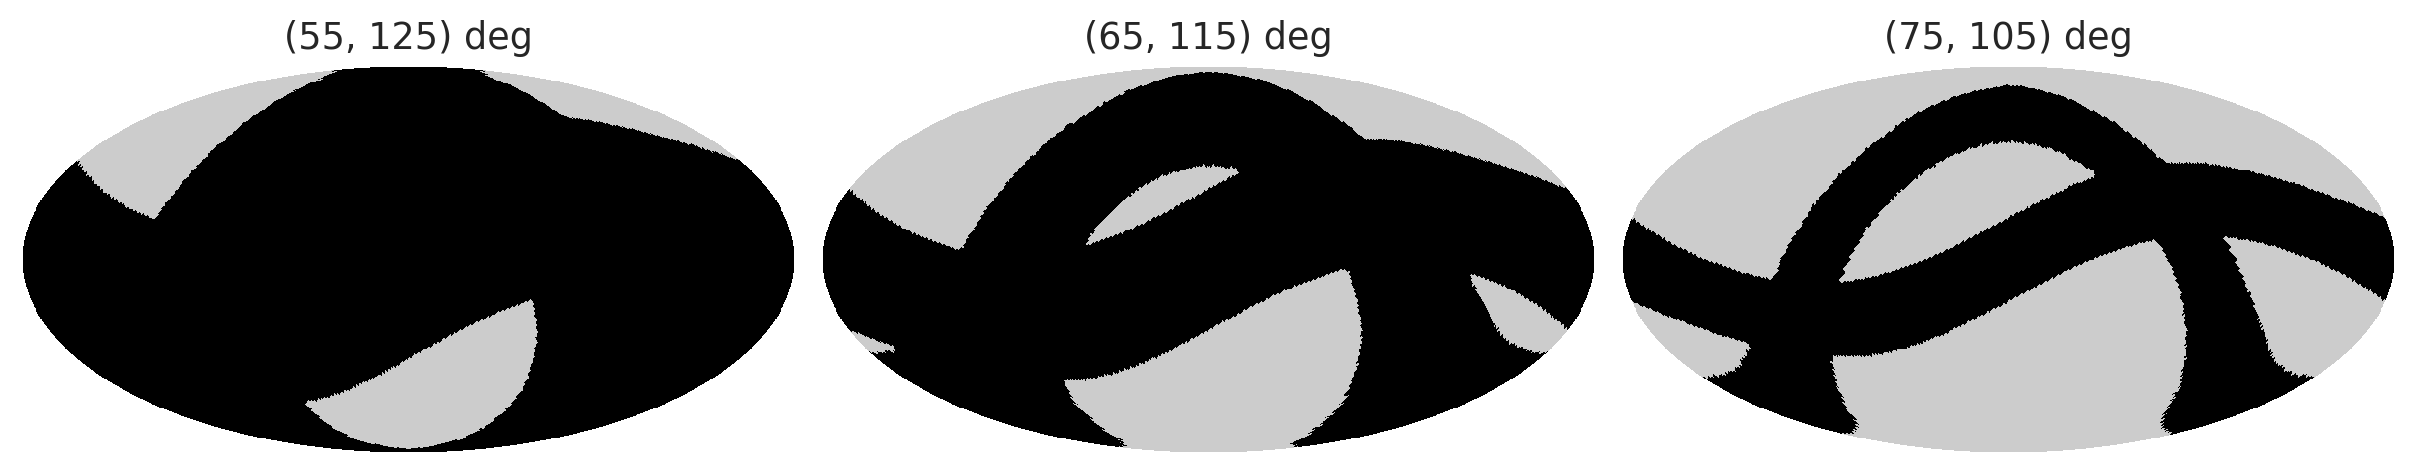
\includegraphics[width=\textwidth]{../examples/report_figures/masks_N64.png}
\caption{The three footprint masks used in the grid ($N_{\rm side}=64$ shown; the
$N_{\rm side}=128$ masks are visually identical, see Table~\ref{tab:fsky}).}
\label{fig:masks64}
\end{figure}

For each of the 18 combinations, we run our C++ QML pipeline (Fisher-matrix estimator,
finite-difference derivatives, conjugate-gradient linear solves via Eigen, following the
method of \citet{Maraio2022} Section~2.3), the \texttt{NaMaster} PCl estimator with its
analytic Gaussian covariance, and an independent \texttt{heracles}-based
catalogue-to-$C_\ell$ pipeline (at $2\times$ the QML/PCl map resolution, with its own
mixing-matrix deconvolution), and save the resulting $EE$/$BB$ power-spectrum estimates
and the QML/PCl covariance (standard-deviation) ratio per multipole to disk.

\section{Log-normal fields and QML validity}
\label{sec:lognormal}

The QML estimator's minimum-variance and unbiasedness properties are formally derived
under the assumption of a Gaussian random field. \texttt{GLASS} instead generates
log-normal fields, which is a more realistic model of the late-time, non-linear matter
and convergence field but formally violates this assumption. We do not repeat that
derivation or its robustness tests here; instead we rely directly on
\citet{Maraio2022}, Section~4.5 (``Non-Gaussian maps'') and their Figure~14, in which the
same QML and PCl estimators are applied to both Gaussian and log-normal (via
\texttt{Flask}) realisations at $N_{\rm side}=256$, and the ratio of PCl to QML
standard deviation is found to be ``virtually identical'' between the two cases. This
demonstrates empirically that QML's variance advantage over PCl persists for log-normal
fields, which is the basis for applying our QML pipeline to \texttt{GLASS}'s
log-normal-field-based mock catalogues in this document.

\section{Results: sky coverage and depth requirements}
\label{sec:results}

\subsection{$N_{\rm side}=64$}

Figure~\ref{fig:sigma64} shows the ratio of PCl to QML standard deviation,
$\sigma_\ell^{\rm PCl}/\sigma_\ell^{\rm QML}$, for the $EE$ and $BB$ blocks, across the
$3\times3$ grid of galaxy density (rows) and footprint (columns). A ratio above unity
means QML is more precise than PCl at that multipole. The narrowest footprint,
$(55,125)^\circ$ ($f_{\rm sky}=15\%$), shows a large QML advantage at low $\ell$ for
both $EE$ and especially $BB$ (up to $\sim\!40\times$ lower variance), consistent with
\citet{Maraio2022}'s Figure~6, where PCl is sub-optimal by $\sim\!20\%$ for $EE$ at
$\ell\lesssim50$ and its $BB$ errors are several times larger than QML's. As the
footprint widens (columns to the right), this advantage shrinks toward unity: once the
mask is close to full-sky, PCl and QML become close to equally precise, since PCl's main
disadvantage is $E$/$B$ mode-mixing and information loss induced by a mask, which
matters less as the unmasked fraction grows.

\begin{figure}[H]
\centering
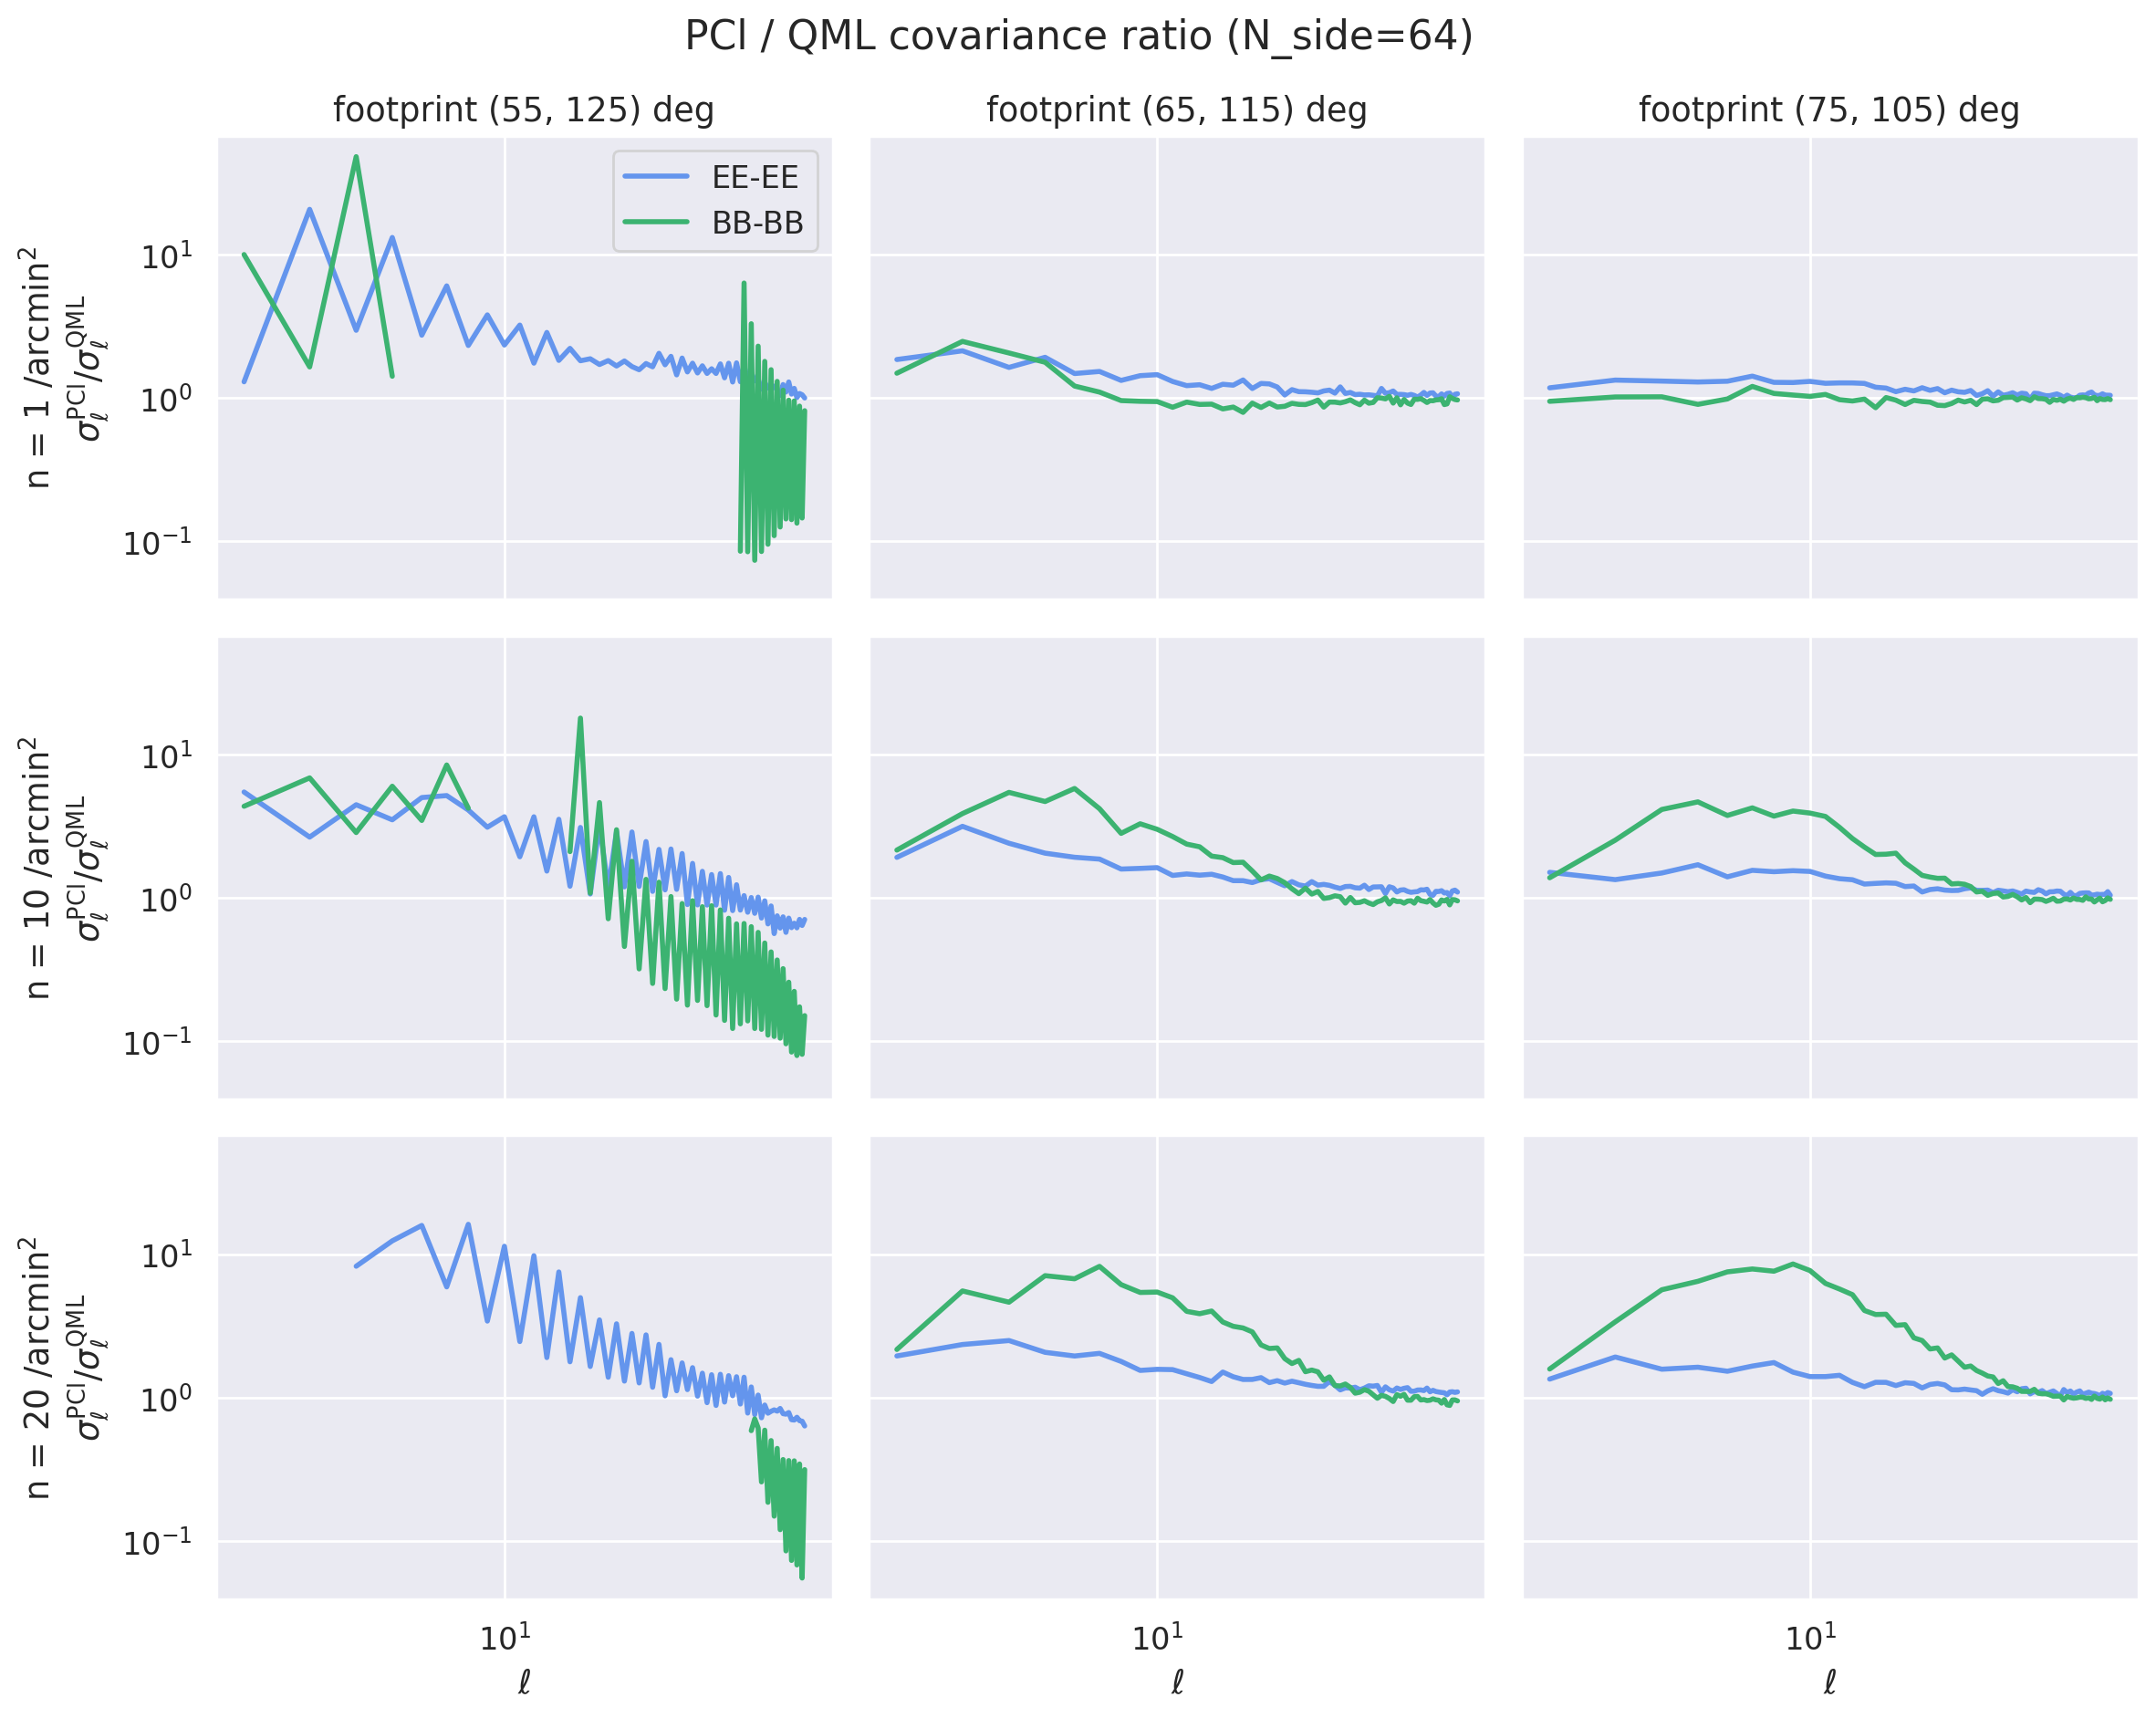
\includegraphics[width=\textwidth]{../examples/report_figures/sigma_ratio_N64.png}
\caption{$N_{\rm side}=64$: ratio of PCl to QML standard deviation for $EE$ (blue) and
$BB$ (green), by galaxy density (rows) and footprint (columns).}
\label{fig:sigma64}
\end{figure}

Figure~\ref{fig:ee64} shows the recovered $EE$ power spectra themselves. All three
estimators track the input theory spectrum well once the footprint is wide enough;
with the narrowest footprint the QML estimate becomes visibly noisier (large
excursions, including formally negative values which appear as gaps/spikes on the
log-log axes) as the ill-conditioned, highly-masked Fisher matrix becomes harder to
invert reliably.

\begin{figure}[H]
\centering
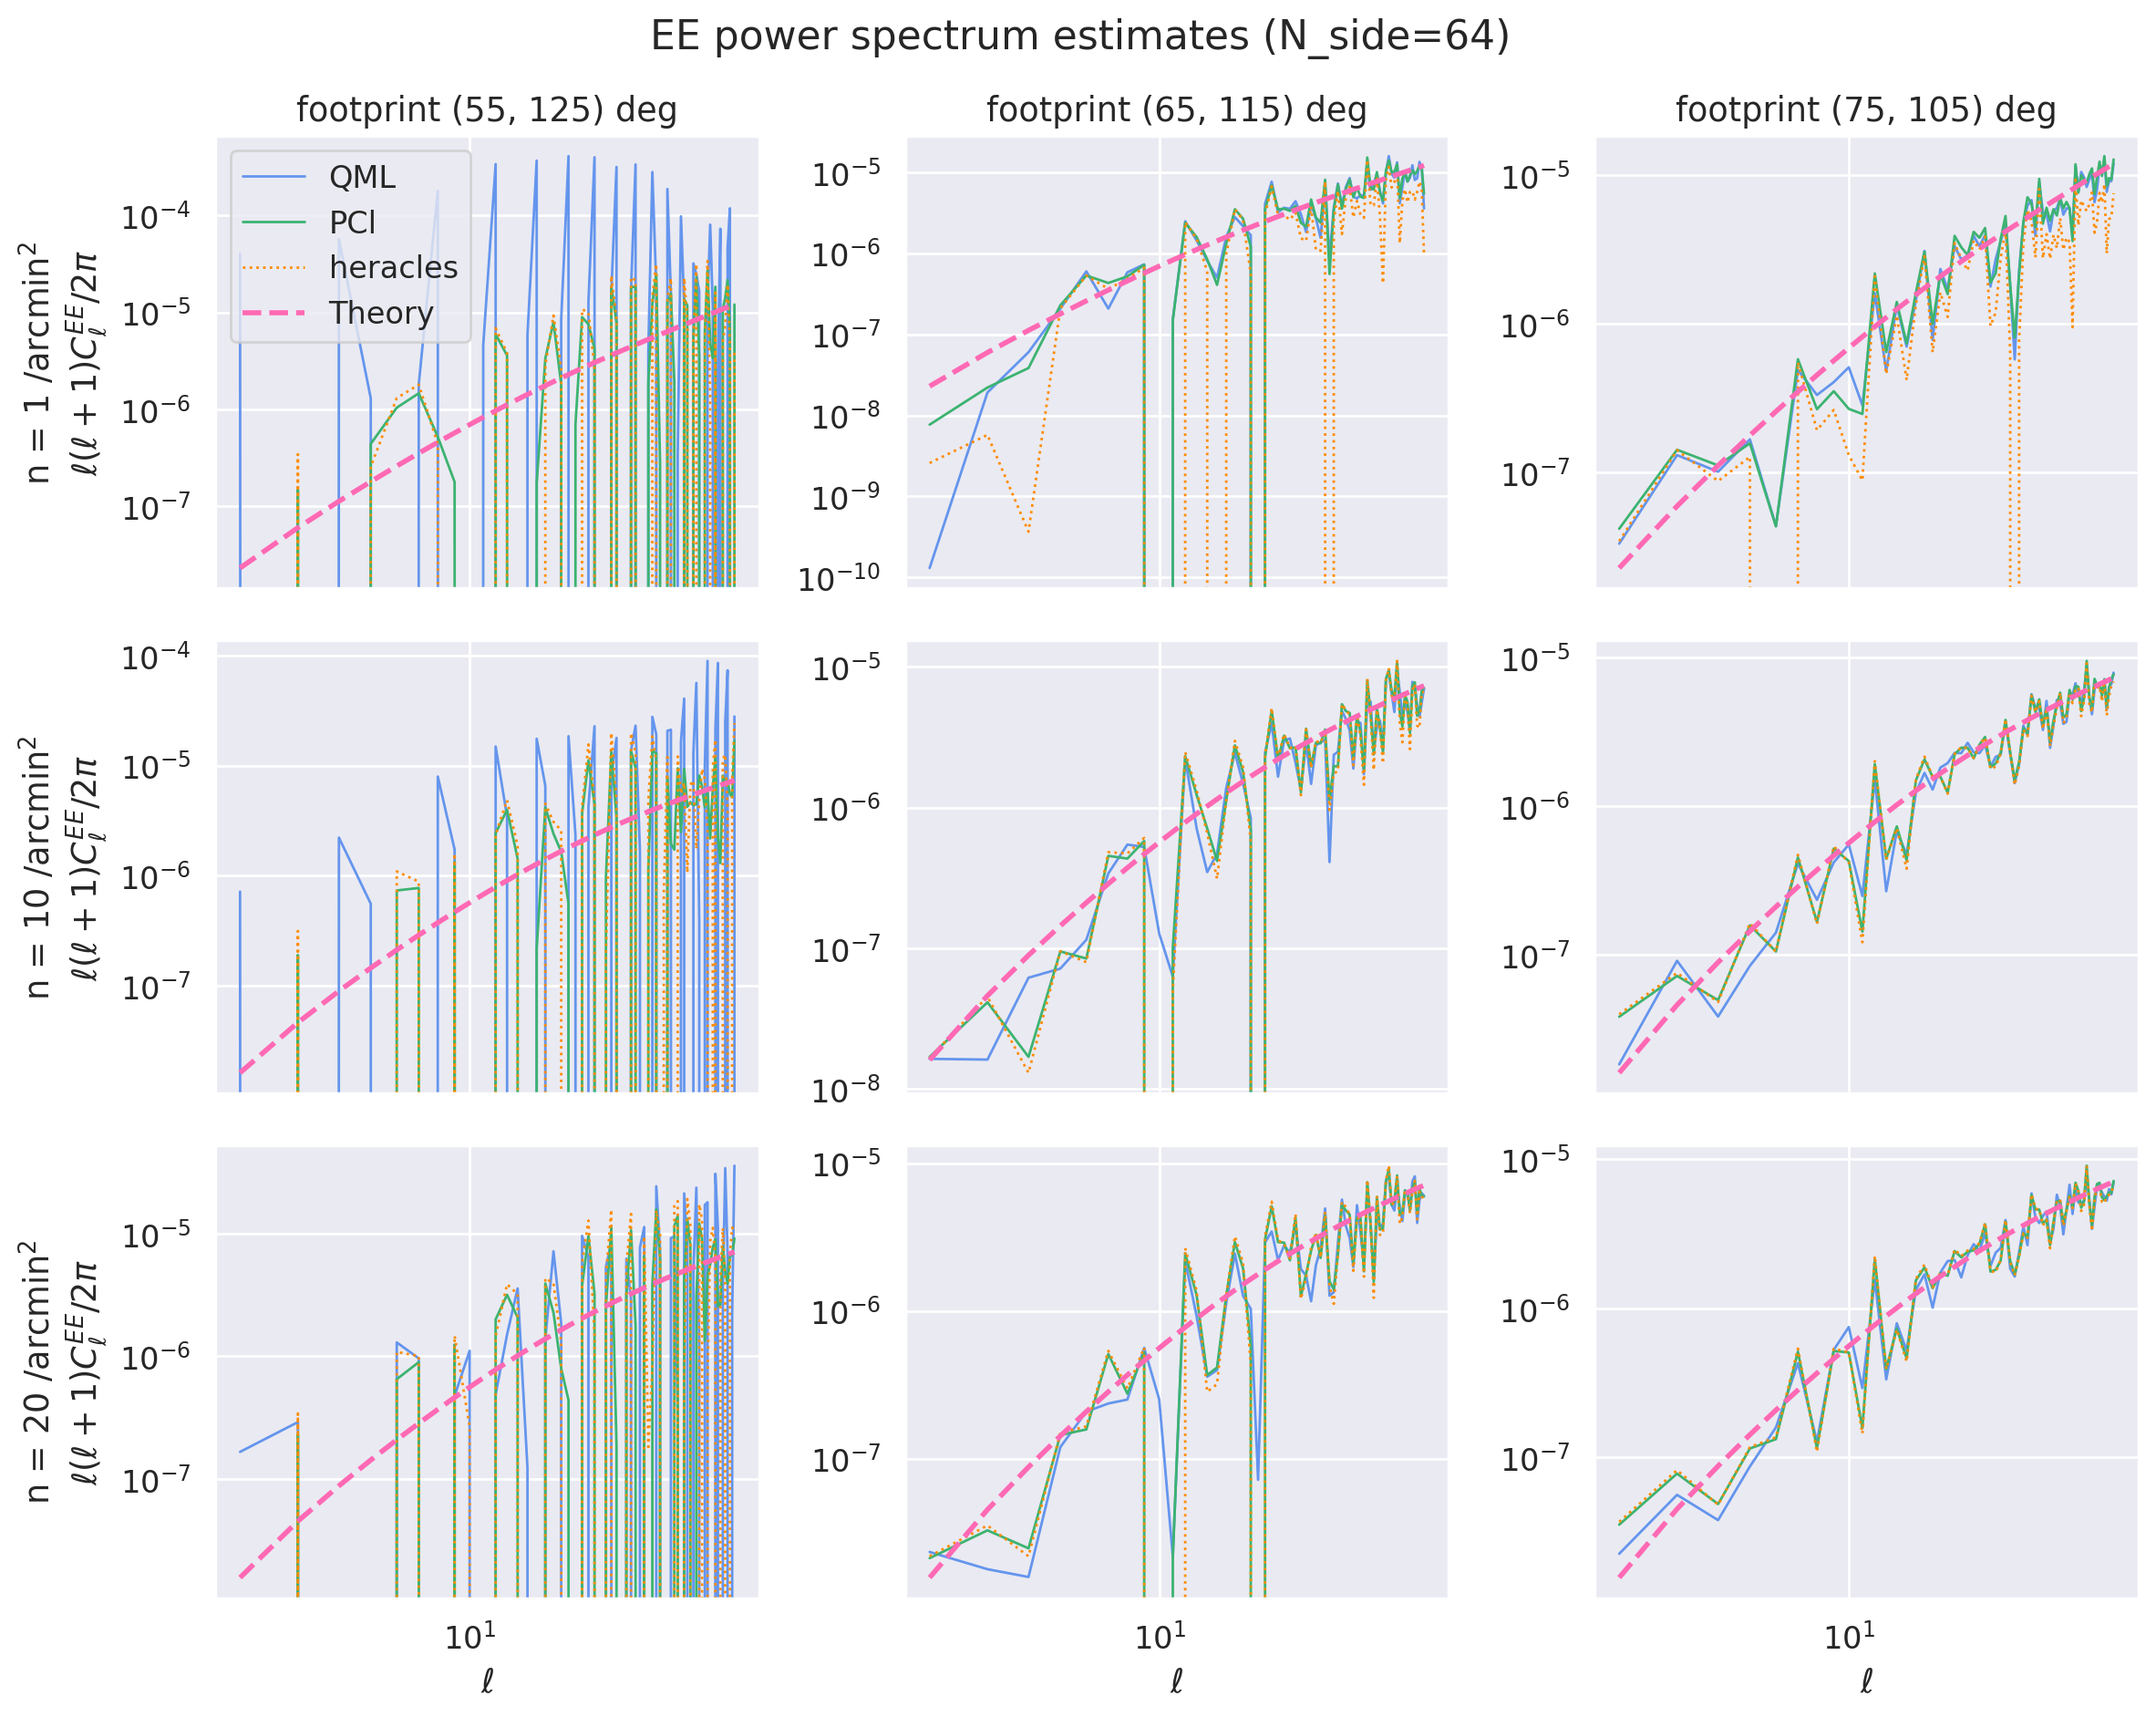
\includegraphics[width=\textwidth]{../examples/report_figures/EE_N64.png}
\caption{$N_{\rm side}=64$: $EE$ power spectrum estimates (QML, PCl, \texttt{heracles},
theory), by galaxy density (rows) and footprint (columns).}
\label{fig:ee64}
\end{figure}

Figure~\ref{fig:bb64} shows the corresponding $BB$ estimates, which have no true
cosmological signal in this simulation and should recover pure shot noise (dashed pink
line) if the estimator is behaving well. Table~\ref{tab:bbnoise64} quantifies this as the
ratio of the mean recovered QML $|C_\ell^{BB}|$ to the theory noise level, both over all
$\ell$ and restricted to $\ell<30$ where leakage is most severe.

\begin{figure}[H]
\centering
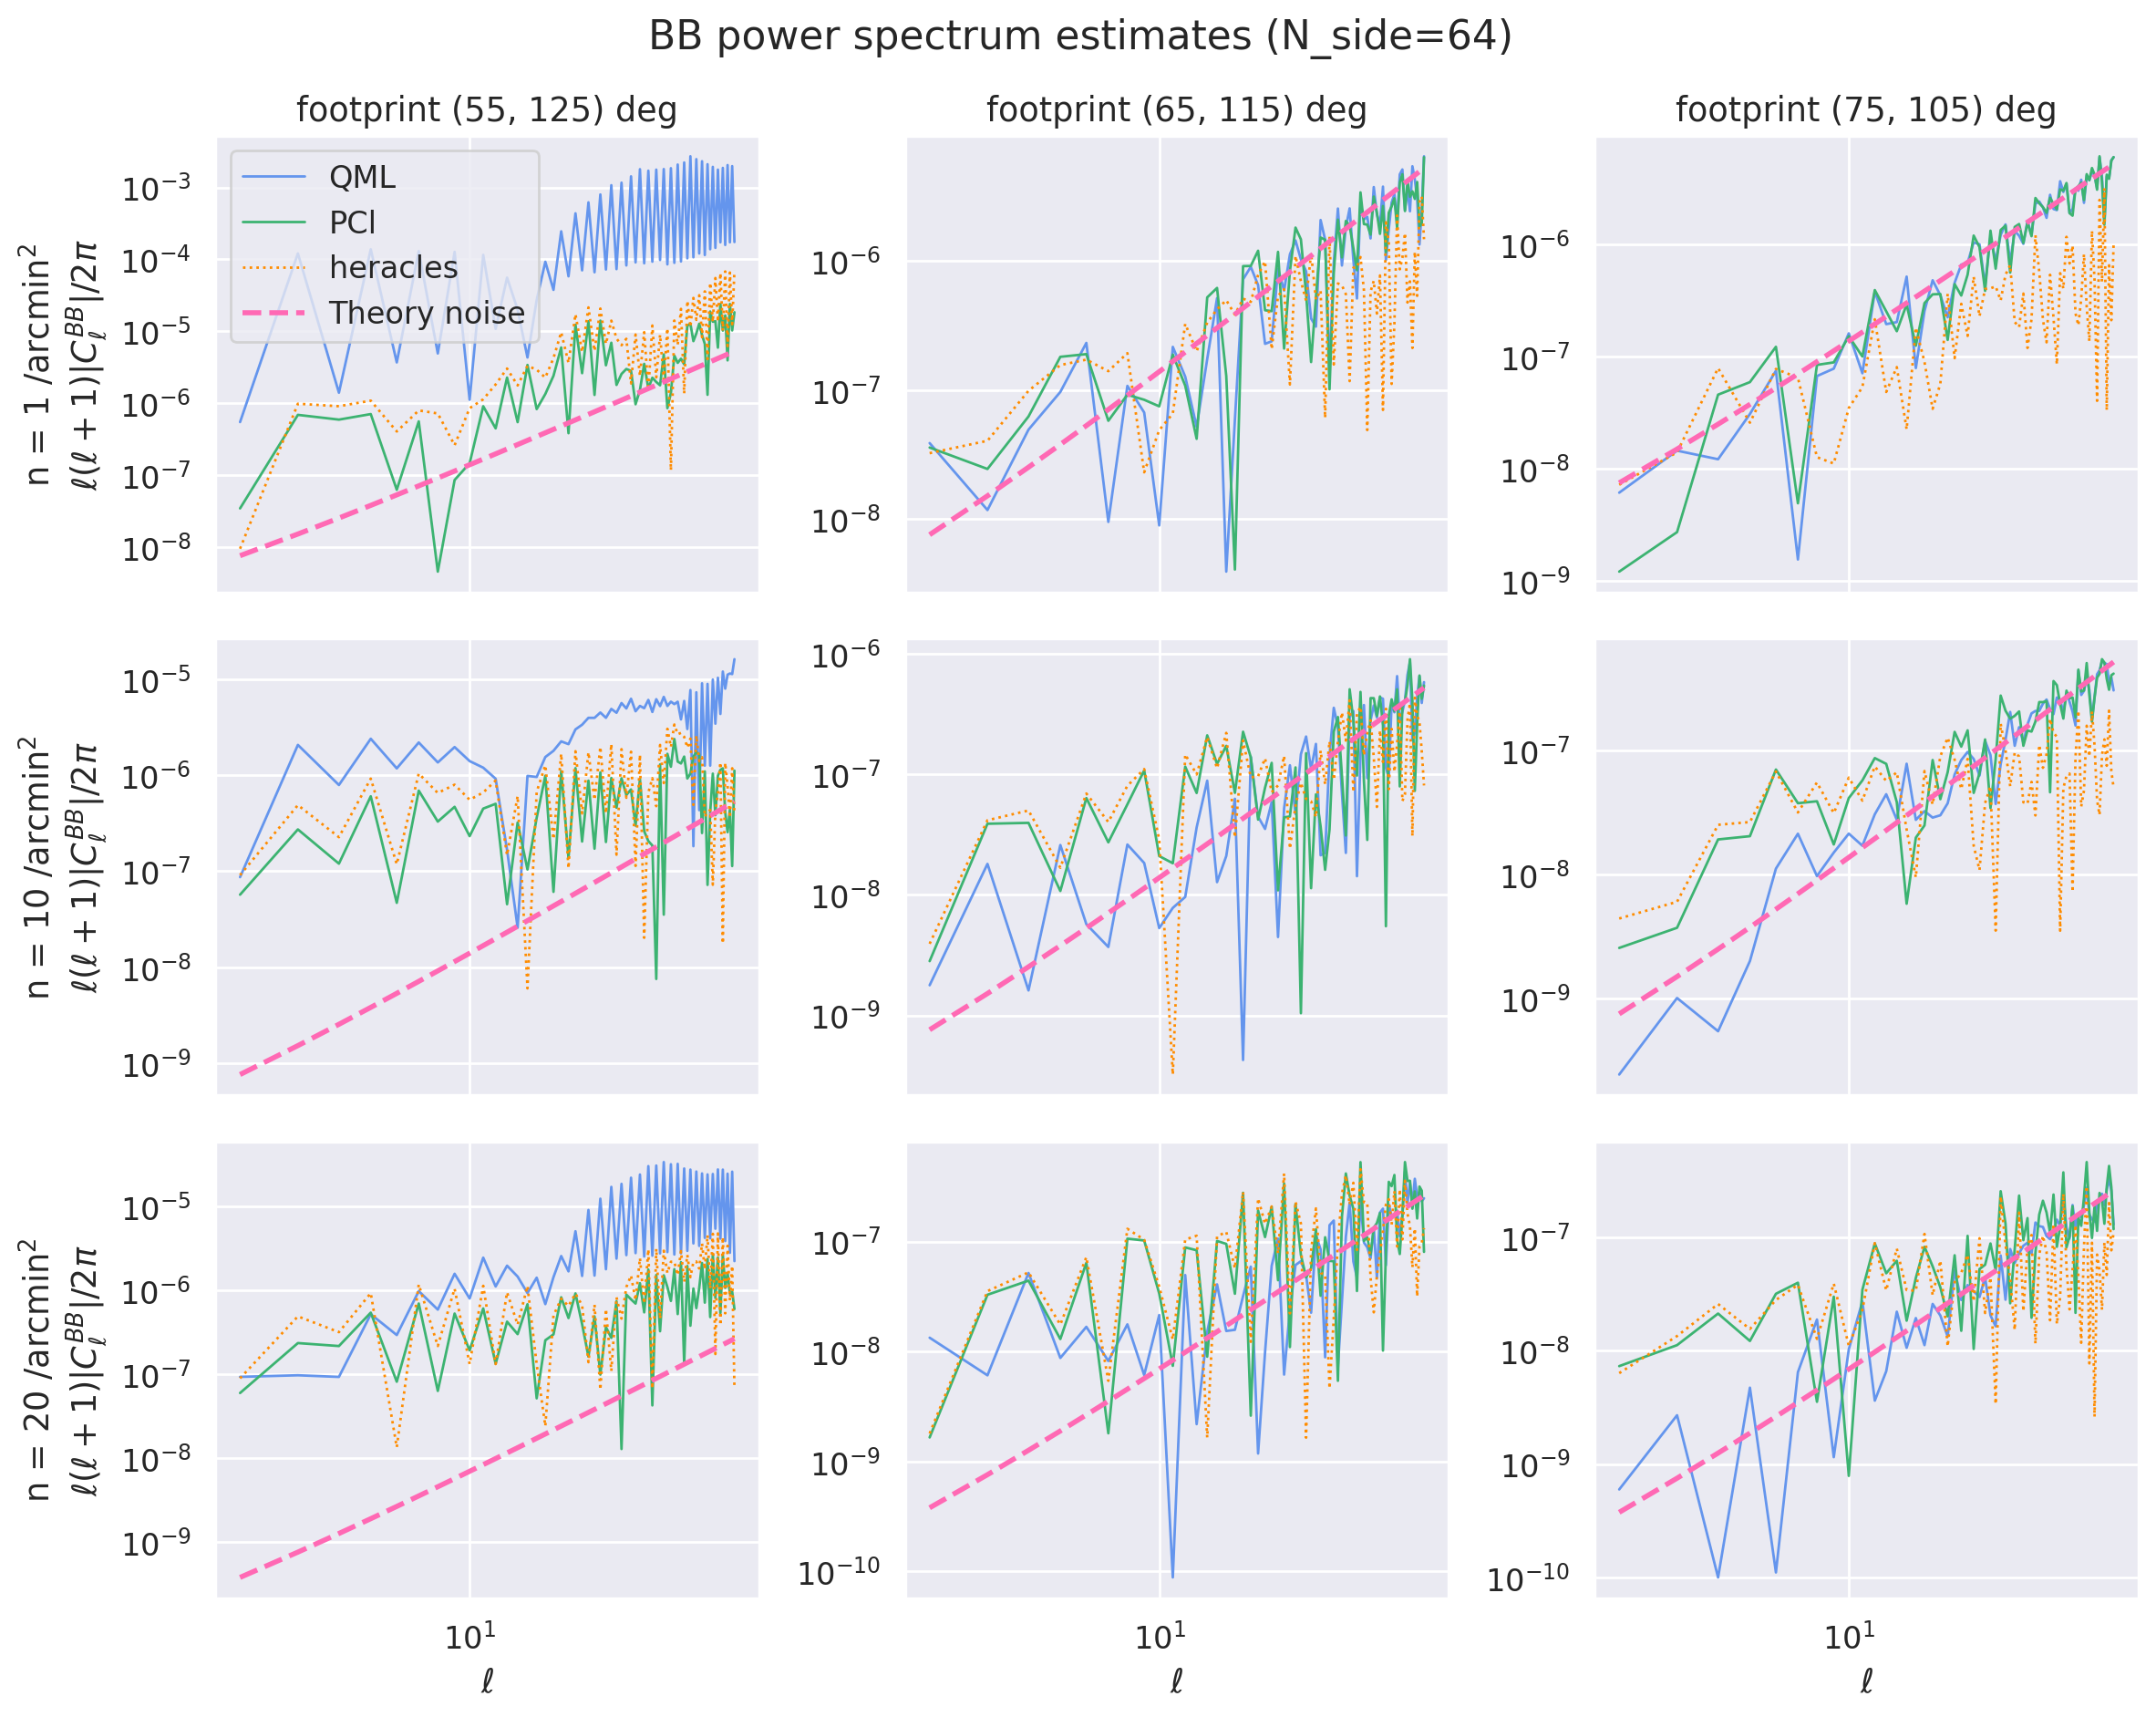
\includegraphics[width=\textwidth]{../examples/report_figures/BB_N64.png}
\caption{$N_{\rm side}=64$: $BB$ power spectrum estimates (QML, PCl, \texttt{heracles},
theory noise), by galaxy density (rows) and footprint (columns).}
\label{fig:bb64}
\end{figure}

\begin{table}[H]
\centering
\begin{tabular}{ccrr}
\toprule
$n\ [\mathrm{arcmin}^{-2}]$ & footprint [deg] & BB/noise ($\ell<30$) & BB/noise (all $\ell$) \\
\midrule
1  & $(55,125)$ & 782.83 & 566.82 \\
1  & $(65,115)$ &   1.22 &   1.01 \\
1  & $(75,105)$ &   0.89 &   0.94 \\
10 & $(55,125)$ & 148.39 &  79.04 \\
10 & $(65,115)$ &   1.76 &   1.36 \\
10 & $(75,105)$ &   1.14 &   1.05 \\
20 & $(55,125)$ & 153.28 & 134.08 \\
20 & $(65,115)$ &   4.66 &   2.69 \\
20 & $(75,105)$ &   1.25 &   1.13 \\
\bottomrule
\end{tabular}
\caption{$N_{\rm side}=64$: ratio of measured QML $|C_\ell^{BB}|$ to the theory shot-noise
level. A ratio close to 1 means the recovered $B$-mode is consistent with pure noise
(a ``clean'' null test).}
\label{tab:bbnoise64}
\end{table}

\subsection{$N_{\rm side}=128$}

The same grid, repeated at twice the resolution, shows the same qualitative behaviour
(Figures~\ref{fig:sigma128}--\ref{fig:bb128}, Table~\ref{tab:bbnoise128}): a strong QML
variance advantage and severe $B$-mode leakage for the narrowest footprint, and
near-unity ratios / noise-consistent $B$-modes once the footprint is wide. The
$B$-mode/noise excess for the narrow footprint is somewhat less extreme at
$N_{\rm side}=128$ than at $N_{\rm side}=64$ (e.g.\ $\sim\!100\times$ vs.\ $\sim\!800\times$
at $n=1\ \mathrm{arcmin}^{-2}$, $\ell<30$), most likely because the extra small-scale
information available at higher $\ell_{\rm max}$ partially dilutes the low-$\ell$
leakage-dominated average, but the qualitative conclusion is unchanged.

\begin{figure}[H]
\centering
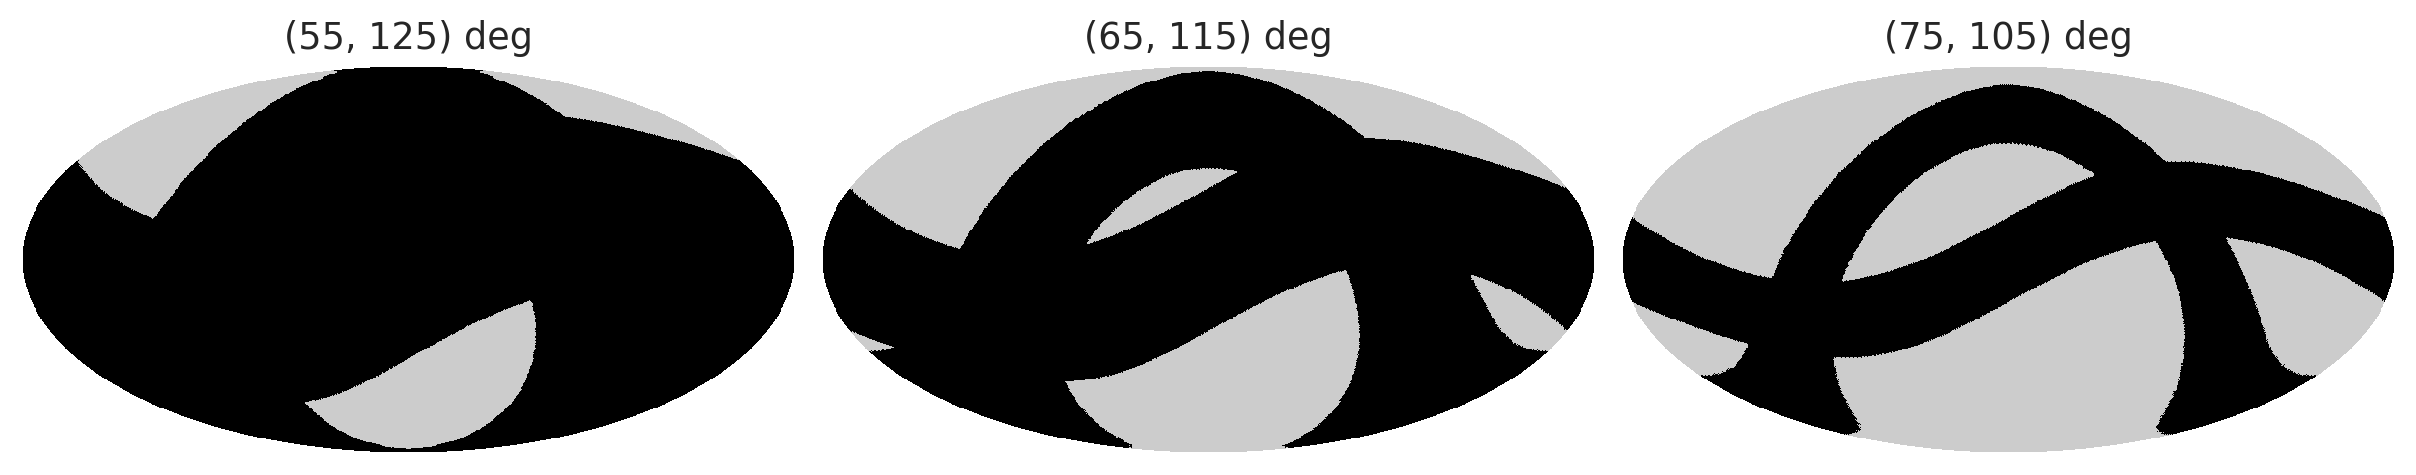
\includegraphics[width=\textwidth]{../examples/report_figures/masks_N128.png}
\caption{The three footprint masks at $N_{\rm side}=128$ (near-identical $f_{\rm sky}$ to
$N_{\rm side}=64$, Table~\ref{tab:fsky}).}
\label{fig:masks128}
\end{figure}

\begin{figure}[H]
\centering
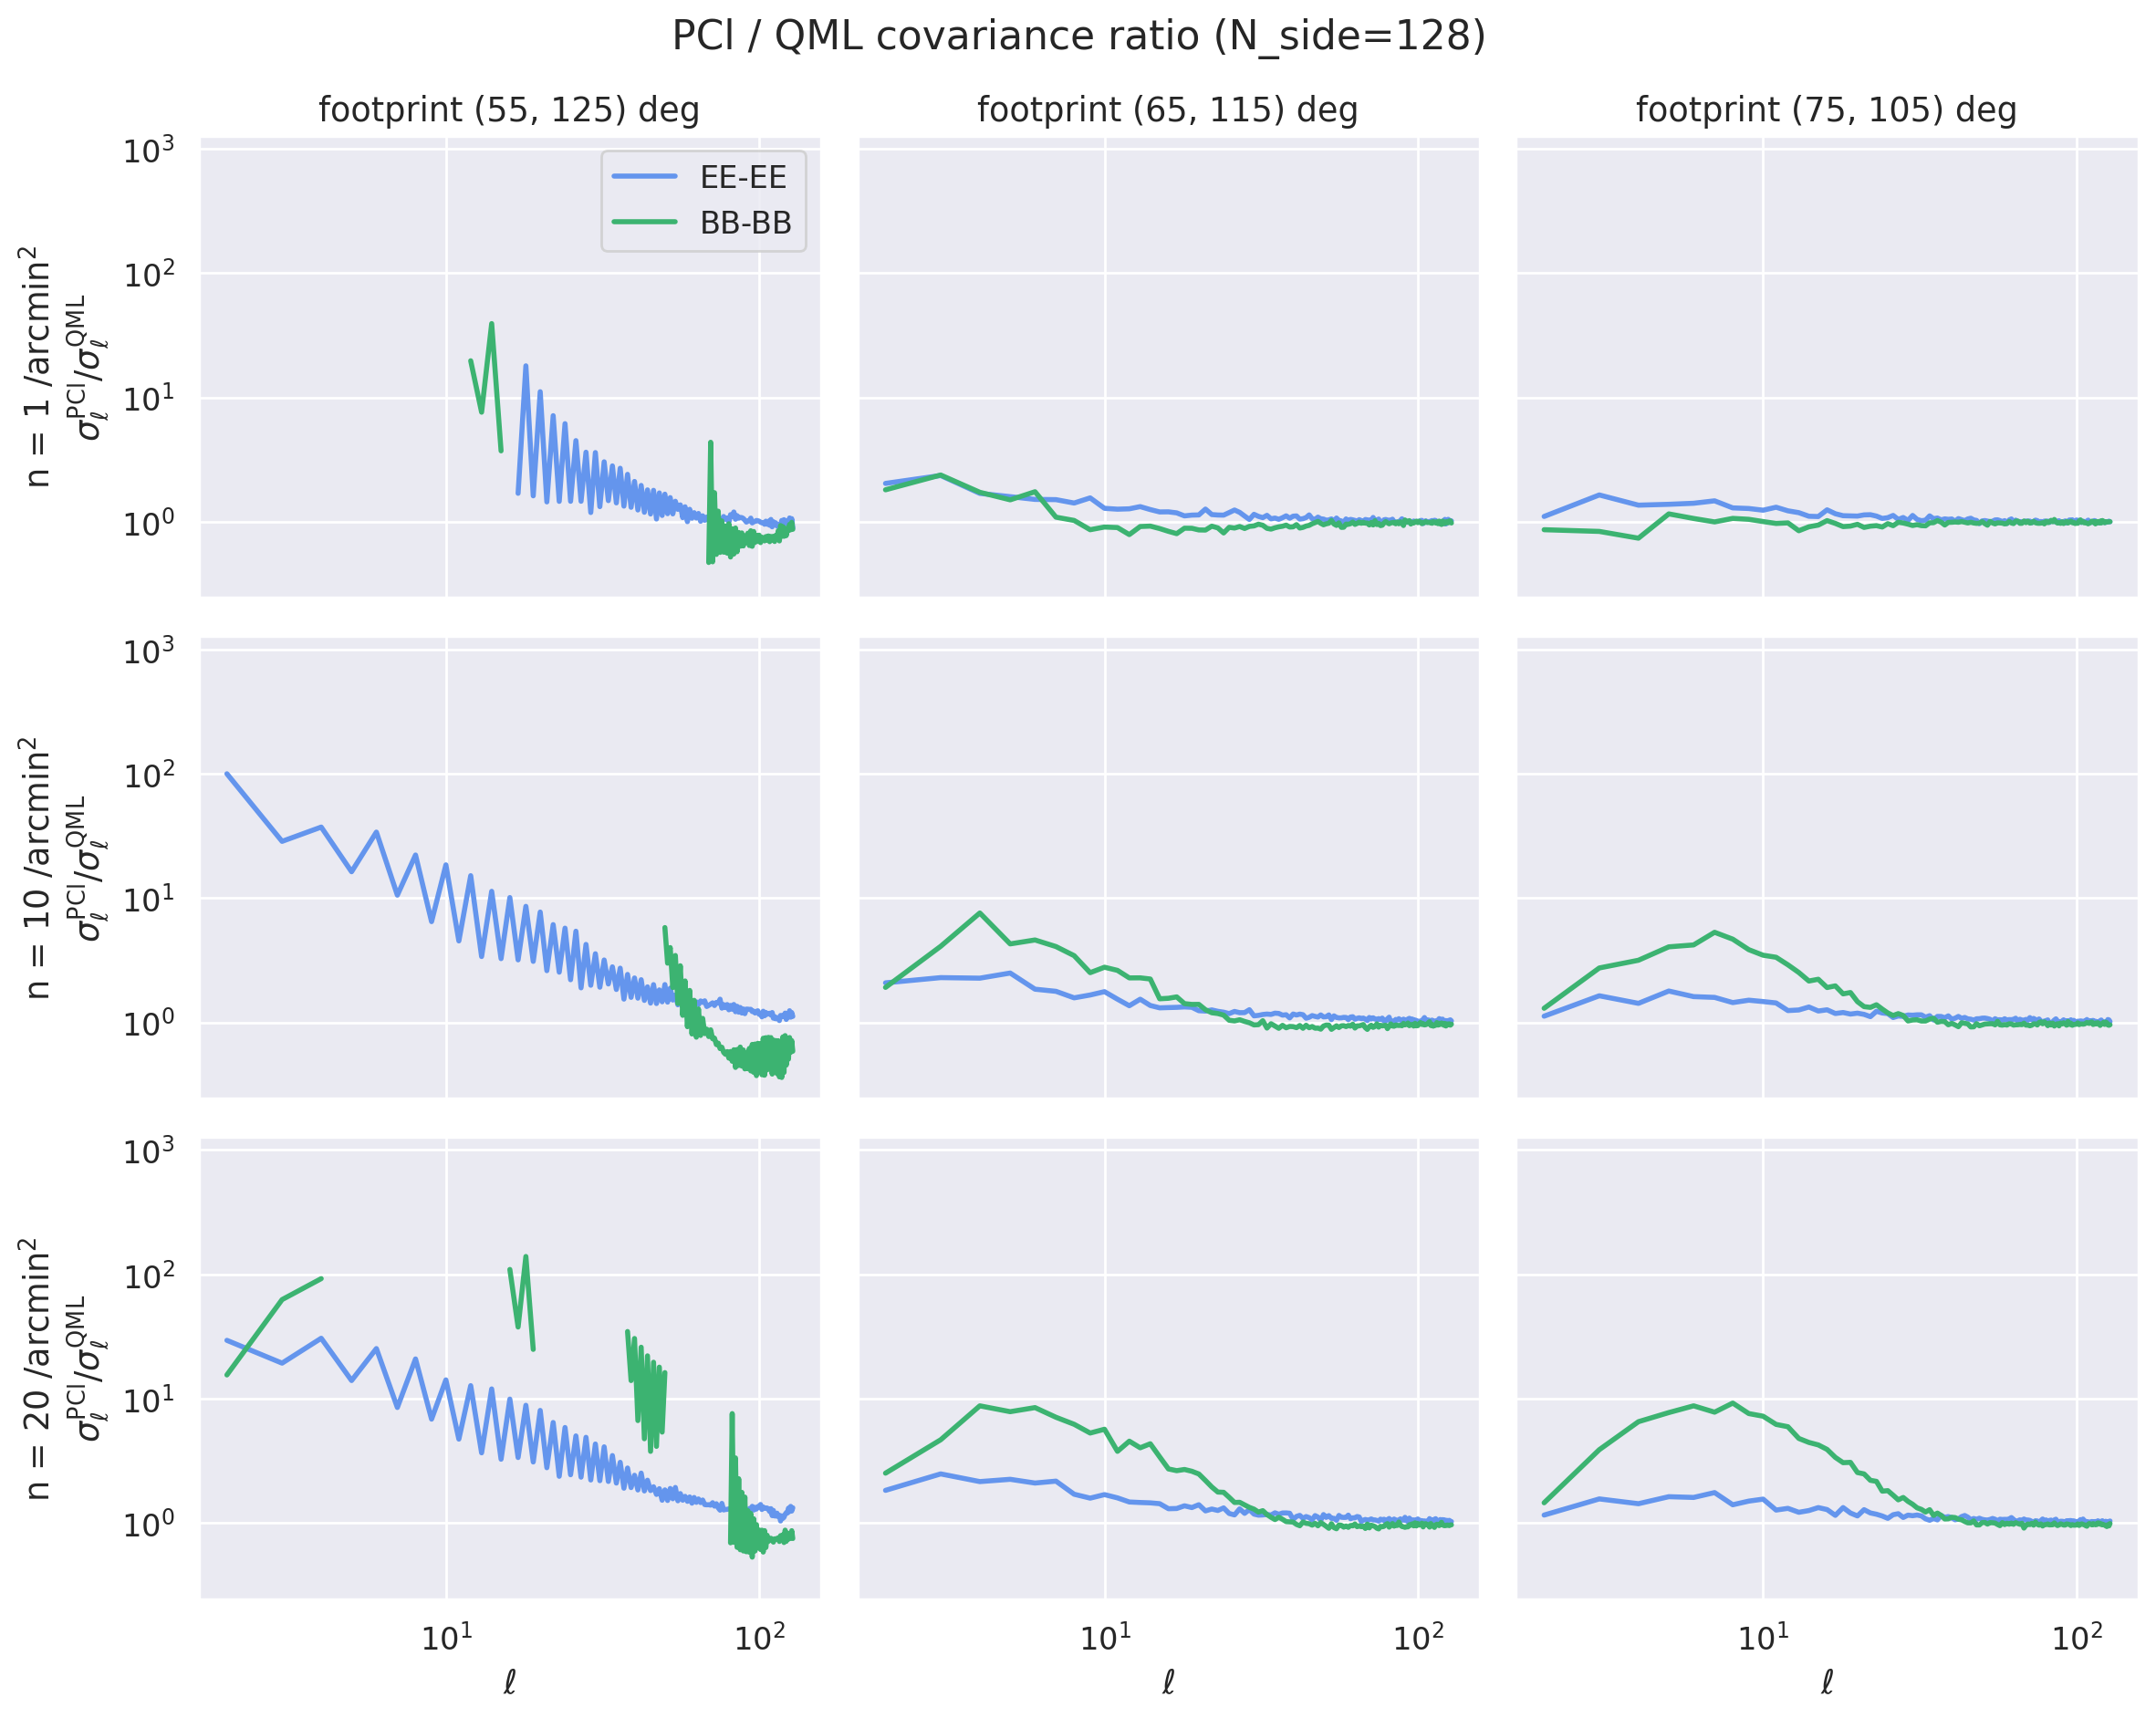
\includegraphics[width=\textwidth]{../examples/report_figures/sigma_ratio_N128.png}
\caption{$N_{\rm side}=128$: ratio of PCl to QML standard deviation for $EE$ (blue) and
$BB$ (green), by galaxy density (rows) and footprint (columns).}
\label{fig:sigma128}
\end{figure}

\begin{figure}[H]
\centering
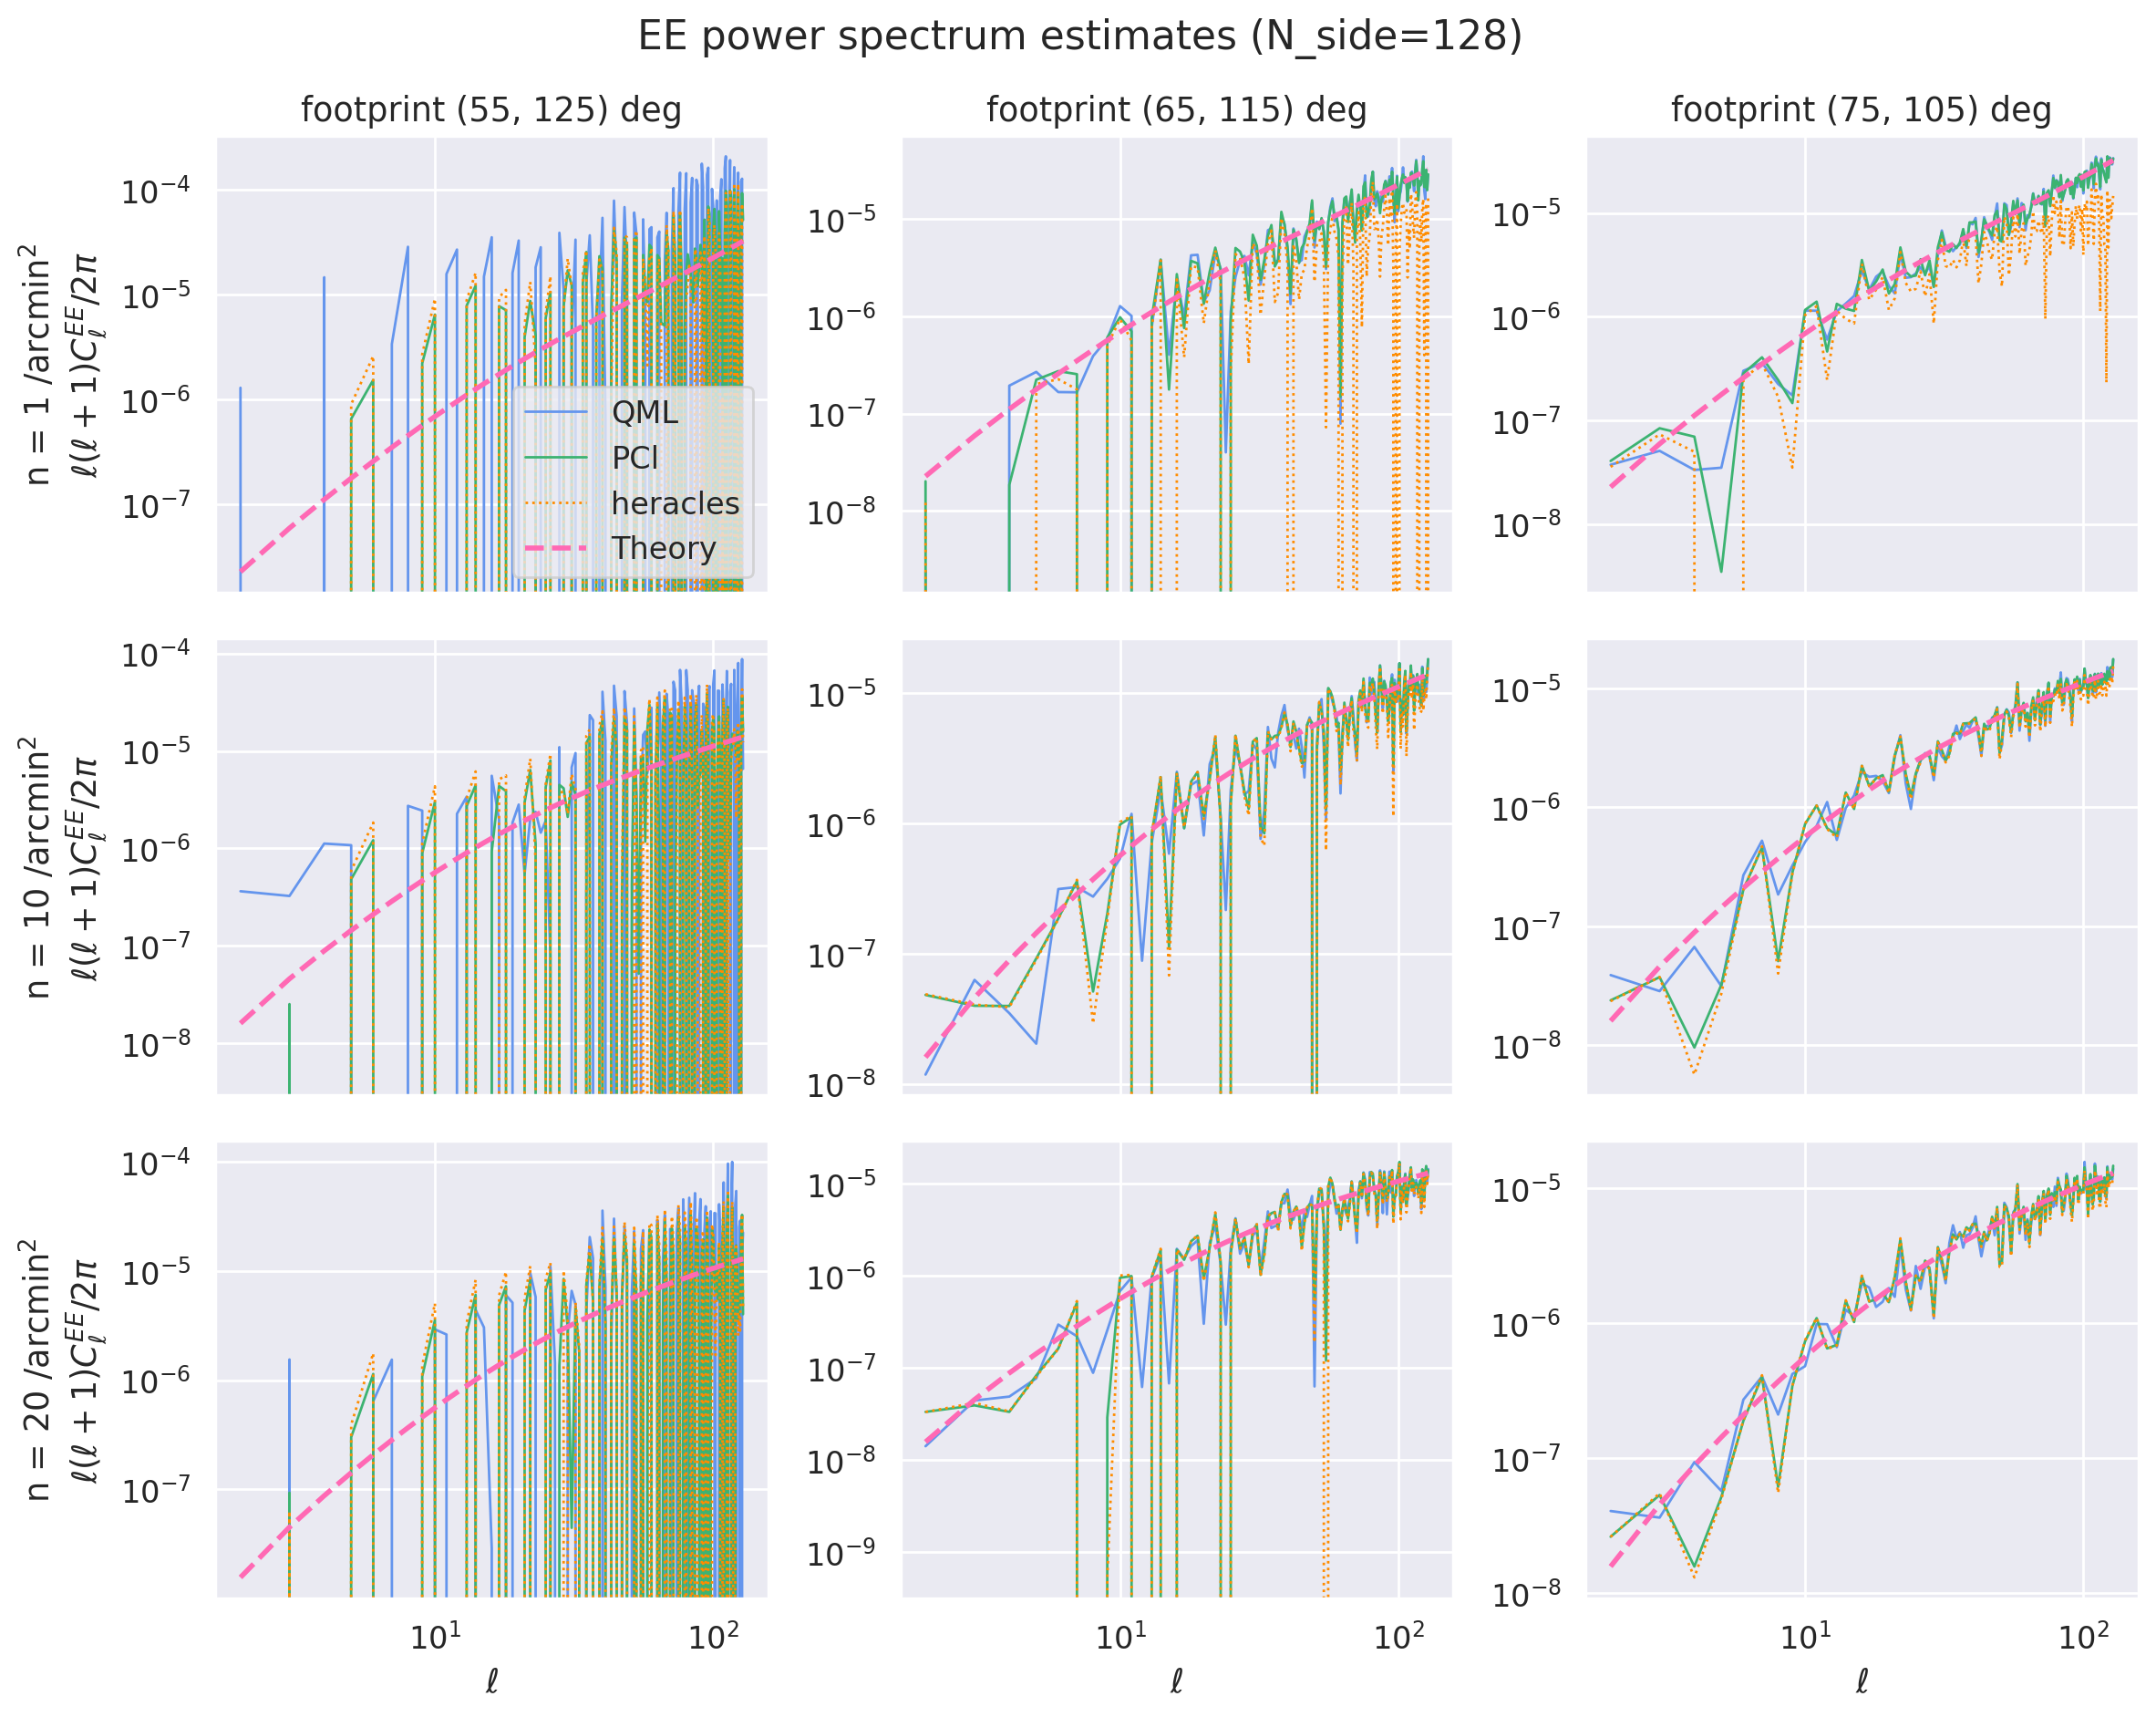
\includegraphics[width=\textwidth]{../examples/report_figures/EE_N128.png}
\caption{$N_{\rm side}=128$: $EE$ power spectrum estimates, by galaxy density (rows) and
footprint (columns).}
\label{fig:ee128}
\end{figure}

\begin{figure}[H]
\centering
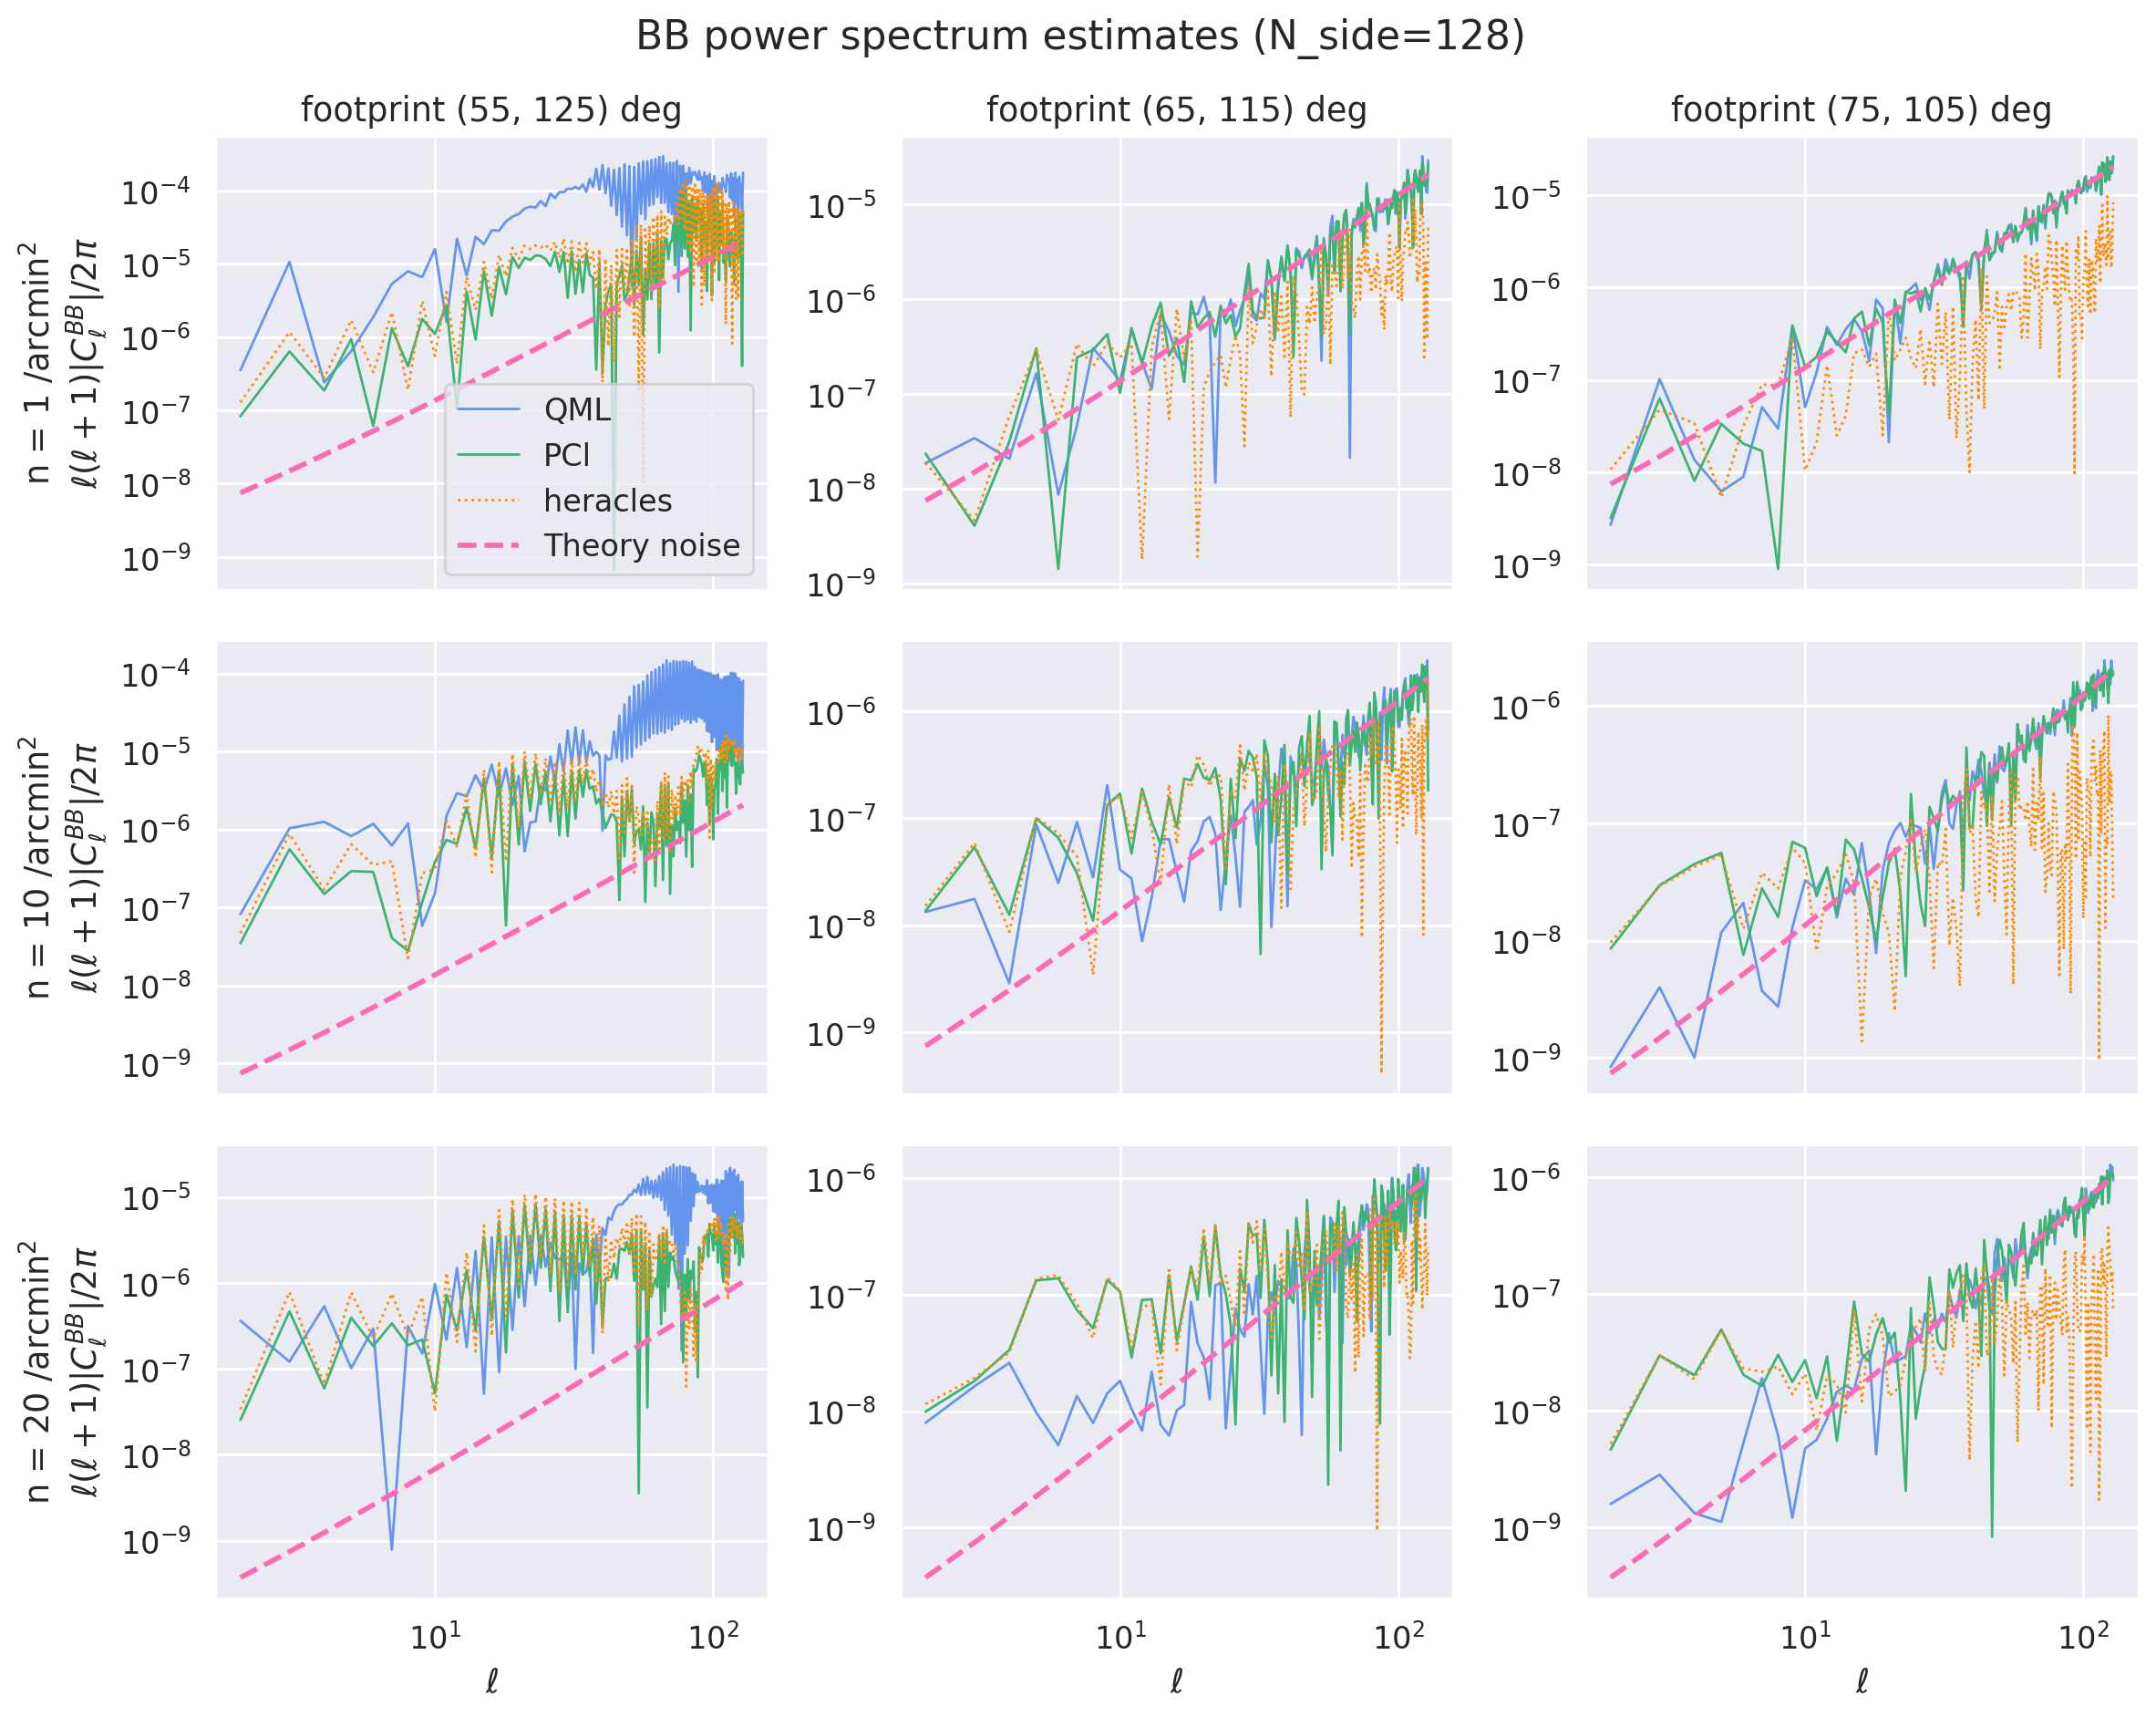
\includegraphics[width=\textwidth]{../examples/report_figures/BB_N128.png}
\caption{$N_{\rm side}=128$: $BB$ power spectrum estimates, by galaxy density (rows) and
footprint (columns).}
\label{fig:bb128}
\end{figure}

\begin{table}[H]
\centering
\begin{tabular}{ccrr}
\toprule
$n\ [\mathrm{arcmin}^{-2}]$ & footprint [deg] & BB/noise ($\ell<30$) & BB/noise (all $\ell$) \\
\midrule
1  & $(55,125)$ & 97.28  & 42.66 \\
1  & $(65,115)$ &  1.45  &  1.07 \\
1  & $(75,105)$ &  1.19  &  1.04 \\
10 & $(55,125)$ & 129.97 & 86.68 \\
10 & $(65,115)$ &  4.19  &  1.70 \\
10 & $(75,105)$ &  1.33  &  1.08 \\
20 & $(55,125)$ & 119.13 & 50.90 \\
20 & $(65,115)$ &  3.93  &  1.68 \\
20 & $(75,105)$ &  1.45  &  1.10 \\
\bottomrule
\end{tabular}
\caption{$N_{\rm side}=128$: ratio of measured QML $|C_\ell^{BB}|$ to the theory
shot-noise level.}
\label{tab:bbnoise128}
\end{table}

\subsection{Overall finding}

Across both resolutions, the grid shows clearly that reproducing \citet{Maraio2022}'s
central result -- that QML's noise is meaningfully below PCl's, particularly for
$B$-modes -- requires \emph{both} a sufficiently wide, well-connected sky footprint
\emph{and} a sufficiently high galaxy number density:
\begin{itemize}
\item \textbf{Coverage controls leakage.} With the narrowest, most fragmented footprint
($f_{\rm sky}\approx15\%$), the recovered $B$-mode exceeds the noise floor by one to
several orders of magnitude at \emph{every} density tested -- mask-induced $E$-to-$B$
leakage dominates regardless of how many galaxies are used, and the QML/PCl variance
ratio, while formally large, is not by itself evidence of a trustworthy measurement.
\item \textbf{Density controls precision.} With the widest footprint
($f_{\rm sky}\approx55\%$), the $B$-mode stays close to the noise floor at every
density, but the absolute size of that noise floor -- and hence how informative a
``consistent with noise'' result is -- only becomes small at the highest density tested
($n=20\ \mathrm{arcmin}^{-2}$).
\item Only the combination of wide coverage \emph{and} high density gives both a low
absolute $B$-mode amplitude and a precise, well-constrained measurement of it, matching
the regime in which \citet{Maraio2022} demonstrate QML's advantage over PCl.
\end{itemize}

\section{The real TR1 catalogue}
\label{sec:tr1}

We repeat the sky-coverage and depth diagnostics of Section~\ref{sec:results} on the
real TR1 Euclid-like shear catalogue, using its effective-coverage HEALPix map degraded
to $N_{\rm side}=256$ and its per-galaxy \texttt{SHE\_WEIGHT}/\texttt{TOM\_BIN\_ID}
columns.

\subsection{Sky coverage}

Figure~\ref{fig:tr1mask} shows the TR1 effective-coverage mask. Its sky fraction is
\[
f_{\rm sky}^{\rm TR1} = 0.371\%,
\]
roughly $40$--$150\times$ smaller than even the narrowest, worst-case footprint used in
our grid ($f_{\rm sky}\approx15\%$, Table~\ref{tab:fsky}), which itself already produced
severe $B$-mode leakage that overwhelmed the shot-noise floor at every density tested
(Tables~\ref{tab:bbnoise64}--\ref{tab:bbnoise128}). By direct extrapolation of that
trend, we would expect a QML (or PCl) analysis of the current TR1 footprint to be
dominated by mask-induced leakage rather than by the underlying signal or shot noise --
i.e.\ the sky coverage of the current TR1 dataset is too small to support a clean QML
null test or precision power-spectrum recovery with this pipeline.

\begin{figure}[H]
\centering
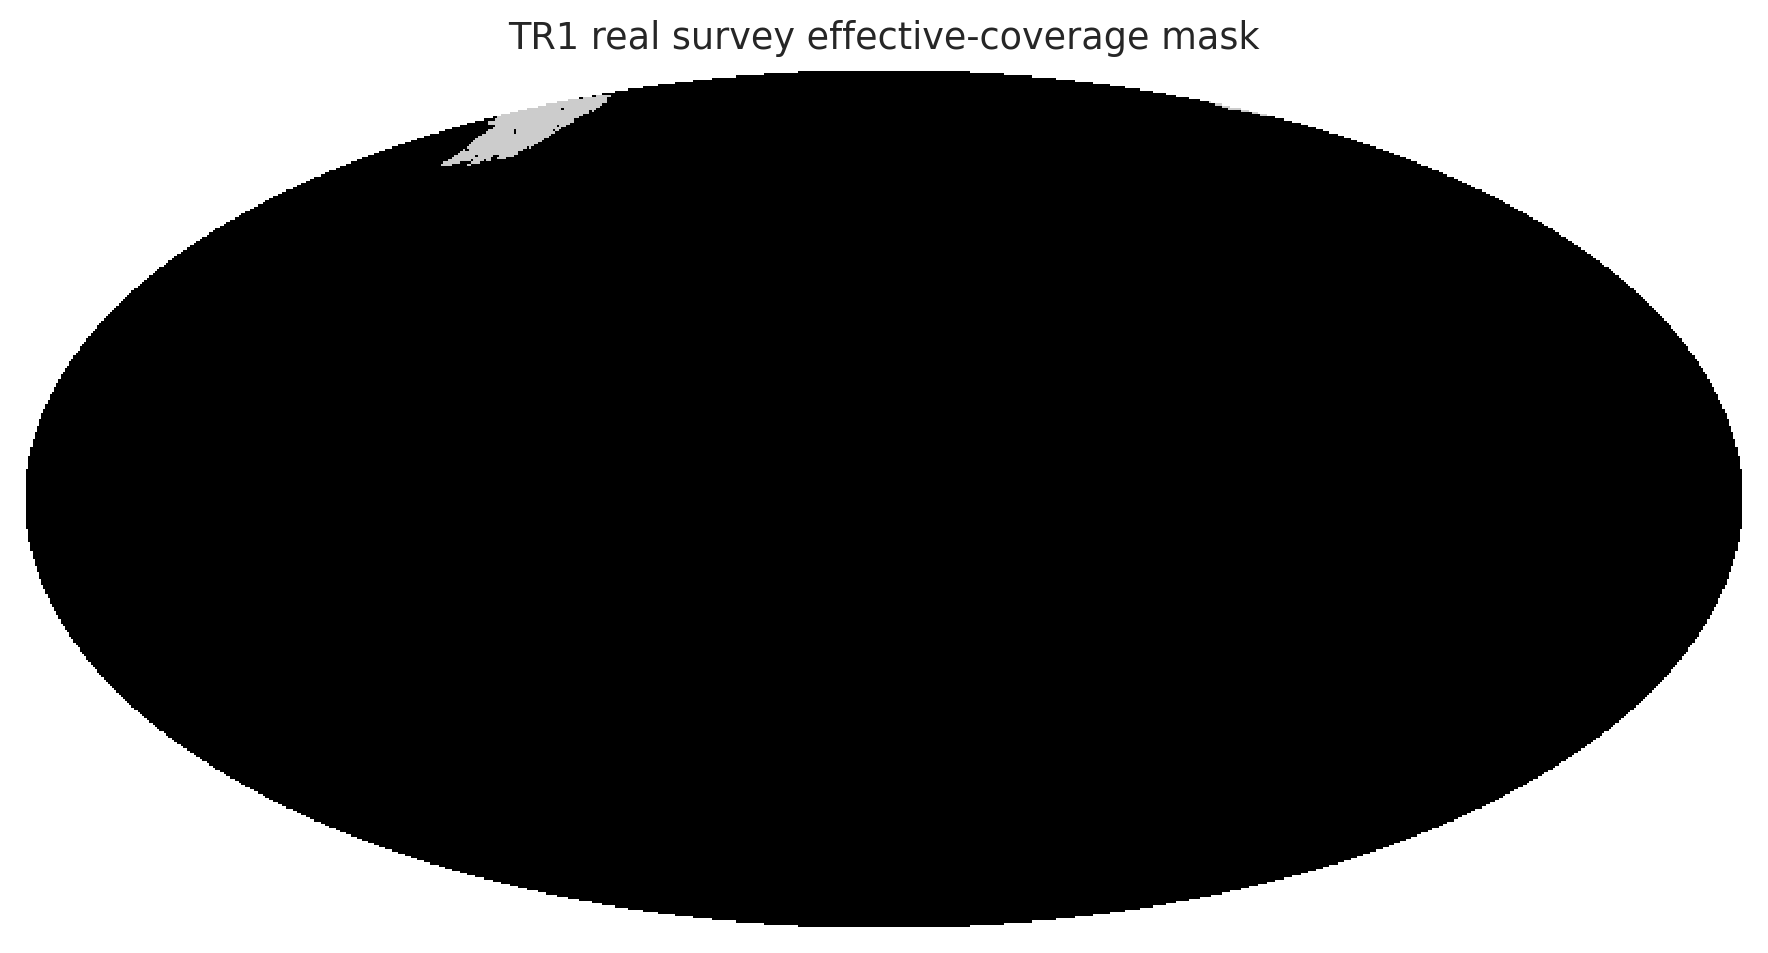
\includegraphics[width=0.7\textwidth]{../examples/report_figures/TR1_mask.png}
\caption{Effective-coverage mask of the real TR1 catalogue, at $N_{\rm side}=256$.
$f_{\rm sky}=0.371\%$.}
\label{fig:tr1mask}
\end{figure}

\subsection{Galaxy density}

Figure~\ref{fig:tr1density} shows the effective galaxy number density
($n_{\rm eff} = (\sum w)^2/\sum w^2$, converted to $\mathrm{arcmin}^{-2}$ over the
unmasked footprint) per tomographic bin and combined across all six bins.

\begin{figure}[H]
\centering
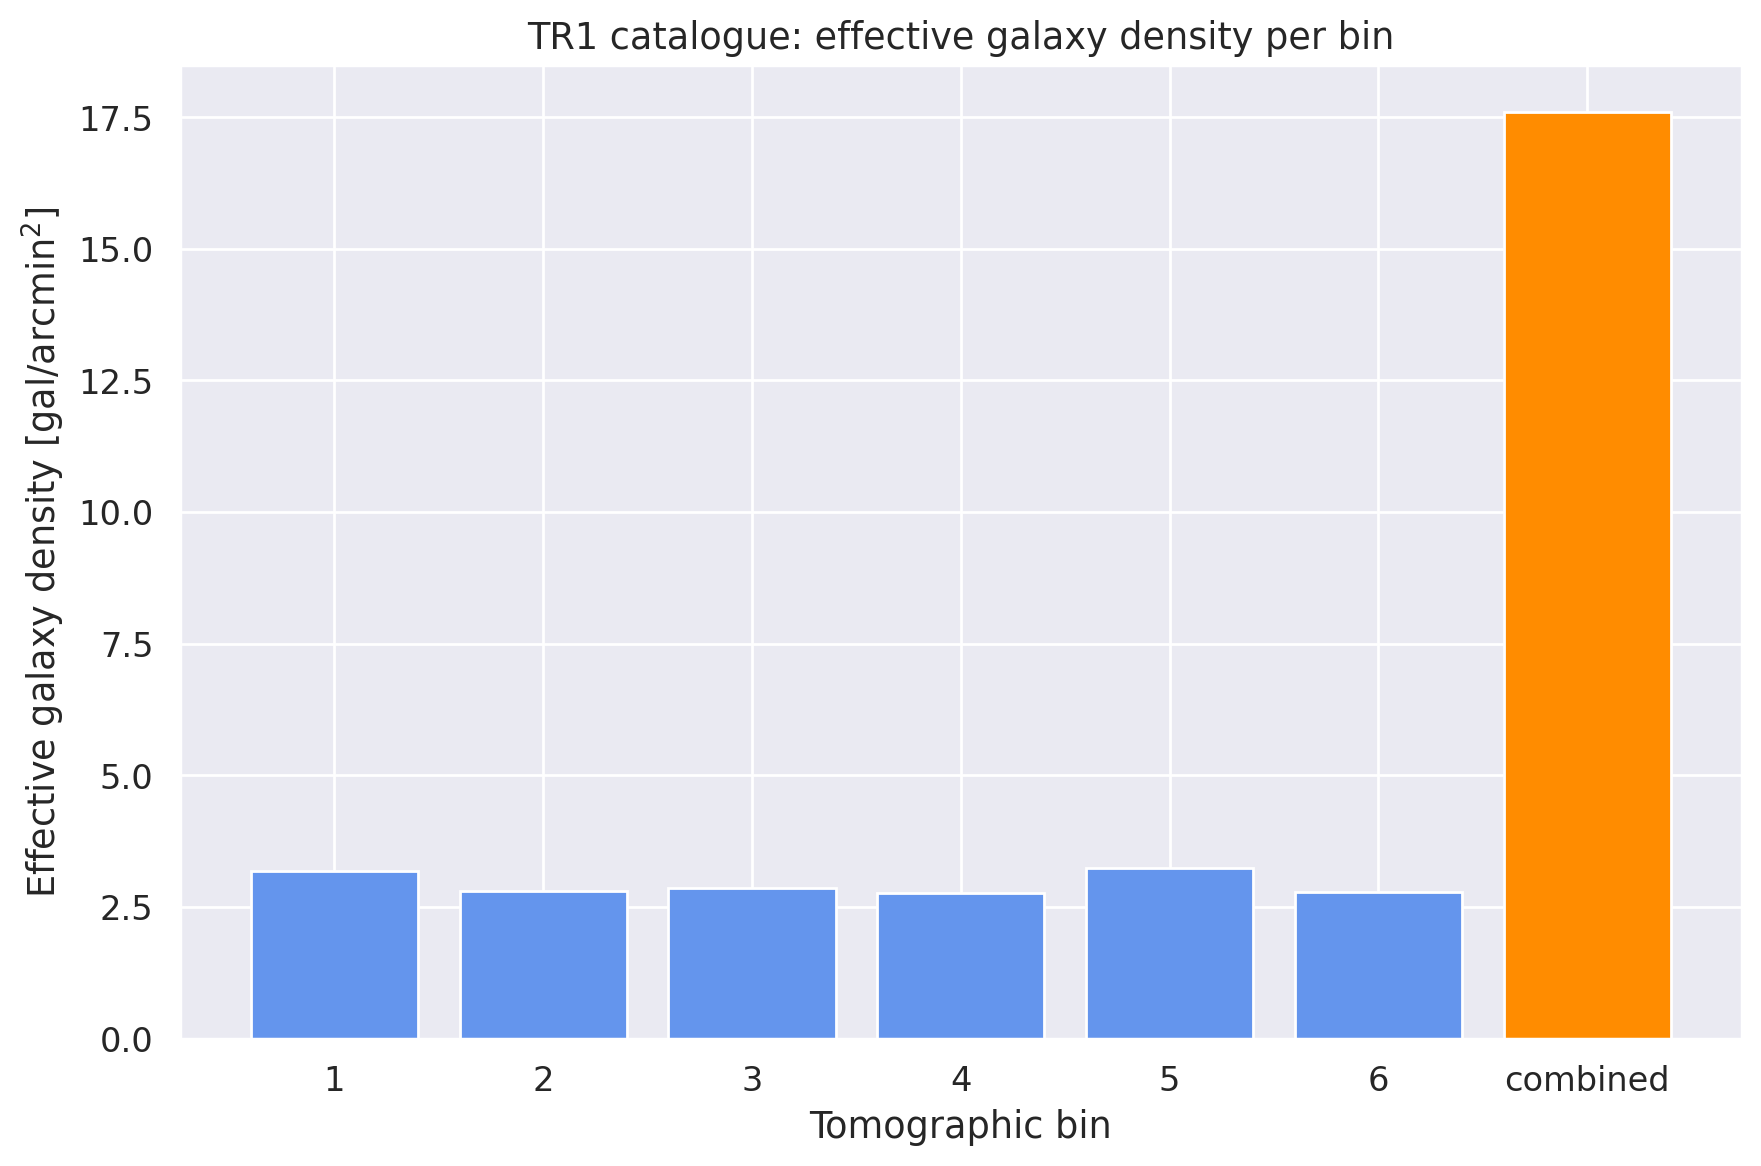
\includegraphics[width=0.7\textwidth]{../examples/report_figures/TR1_density_per_bin.png}
\caption{TR1 catalogue effective galaxy density per tomographic bin (blue) and combined
across all bins (orange).}
\label{fig:tr1density}
\end{figure}

The per-bin densities are all in the range $2.77$--$3.25\ \mathrm{arcmin}^{-2}$
(combined: $17.6\ \mathrm{arcmin}^{-2}$ across all six bins) -- almost exactly the
$n=1$--$10\ \mathrm{arcmin}^{-2}$ range of our grid, and directly comparable to the
$\bar n=3\ \mathrm{arcmin}^{-2}$ per-tomographic-bin case in \citet{Maraio2022}
Section~4.3.1. Unlike the coverage deficit above, this depth is \emph{not} the limiting
factor: our grid shows that a density of a few galaxies per square arcminute is
perfectly workable for QML \emph{provided the footprint is wide enough}
(Tables~\ref{tab:bbnoise64}--\ref{tab:bbnoise128}, $(65,115)^\circ$ and $(75,105)^\circ$
columns, $n=1$ and $n=10\ \mathrm{arcmin}^{-2}$ rows give BB/noise (all $\ell$) ratios
between $0.94$ and $1.70$).

\subsection{Feasibility of a per-bin analysis}

Combining the two findings above: the bottleneck for applying this QML pipeline to a
TR1-like survey on a per-tomographic-bin basis is sky coverage, not galaxy density. Our
$N_{\rm side}=128$, $n=1\ \mathrm{arcmin}^{-2}$ grid point is a reasonable proxy for a
single TR1-like tomographic bin at higher resolution, and it already achieves a
noise-consistent $B$-mode (BB/noise within $\sim\!45\%$ of unity, including at
$\ell<30$) once $f_{\rm sky}\gtrsim30\%$ (Table~\ref{tab:bbnoise128}). This suggests
that, once the observed footprint of a TR1-like survey is enlarged from its current
$0.371\%$ to the tens-of-percent level, a per-bin ($2$--$3\ \mathrm{arcmin}^{-2}$) QML
analysis at $N_{\rm side}=128$ should be achievable with the precision and leakage
control demonstrated here, without needing to combine tomographic bins to boost the
density further.

\section{Conclusion}

Using \texttt{GLASS} log-normal mock weak-lensing catalogues, whose validity as an input
to the QML estimator is supported by the Gaussian/log-normal comparison in
\citet{Maraio2022} Section~4.5, we reproduce that paper's central finding that QML
recovers a lower-variance, leakage-free $B$-mode null test than PCl, but only once both
sky coverage and galaxy density are adequate. Applying the same diagnostics to the real
TR1 catalogue shows its current sky coverage ($f_{\rm sky}=0.371\%$) is far too small for
a reliable QML (or PCl) analysis, while its per-bin galaxy density
($\approx 2.8$--$3.2\ \mathrm{arcmin}^{-2}$) already lies in a workable regime. A
per-tomographic-bin QML power-spectrum analysis of a TR1-like survey therefore looks
feasible at $N_{\rm side}=128$, contingent mainly on enlarging the observed footprint
rather than on combining tomographic bins for extra depth.

\begin{thebibliography}{9}
\bibitem[Maraio, Hall \& Taylor(2022)]{Maraio2022}
A.~Maraio, A.~Hall, A.~N.~Taylor,
\emph{Testing Quadratic Maximum Likelihood estimators for forthcoming Stage-IV weak
lensing surveys},
MNRAS \textbf{000}, 1--14 (2022), arXiv:2207.10412.
\end{thebibliography}

\end{document}
